\clearpage
\section{Invariant mass spectra}
\label{sec:results}

The observed dielectron mass spectrum together with the predicted standard model backgrounds and the integral of the mass spectrum are shown in figure~\ref{mass_2016} (\ref{mass_2017})for the barrel-barrel and barrel-endcap channels and combined channels in 2016 (2017).
In Figure \ref{massratio_2016} (\ref{massratio_2017}), the ratio of observed dielectron mass spectrum in signal region for the barrel-barrel, barrel-endcap and sum of the barrel-barrel and the barrel-endcap together is shown with different binning in 2016 (2017).
The following systematic uncertainties sources are considered.

\begin{itemize}
  \item[$\bullet$] normalization to Z peak: 1\% uncertainty is considered on the normalization factor estimated from Z peak in 2016. In 2017 2\% (4\%) uncertainty is considered for barrel-barrel (barrel-endcap).
  \item[$\bullet$] pileup reweighting: scaling the minimum bias cross section up/down by 4.6\%
  \item[$\bullet$] DY PDF: relative mass dependent uncertainty from DY PDF (see Figure \ref{fig:pdf_rel_uncert})
  \item[$\bullet$] cross section of background processes:7\% uncertainty is considered on the cross section of the Non-DY background estimated from MC for different processes.
  \item[$\bullet$] jets: 50\% uncertainty is considered on fake jet estimation
  \item[$\bullet$] electron energy scale: 2\% in Barrel-Barrel and 1\% in Barrel-Endcap (for mass $>120$)
  \item[$\bullet$] HEEP ID scale factor: For barrel it is 1\%  below 90 GeV and 1-3\% linearly increase for 90GeV-1TeV range and 3\% for higher than 1 TeV. For endcap it is 1\% below 90 GeV and 1-4\% linearly increase for 90GeV-300 GeV and 4\% for higher than 300 GeV in 2016. In 2017 it is the same for barrel, for endcap it is 2\% below 90 GeV and 1-5\% linearly increase for 90GeV-300 GeV and 5\% for higher than 300 GeV.
\end{itemize}


\begin{figure}[ht]
  \begin{center}
    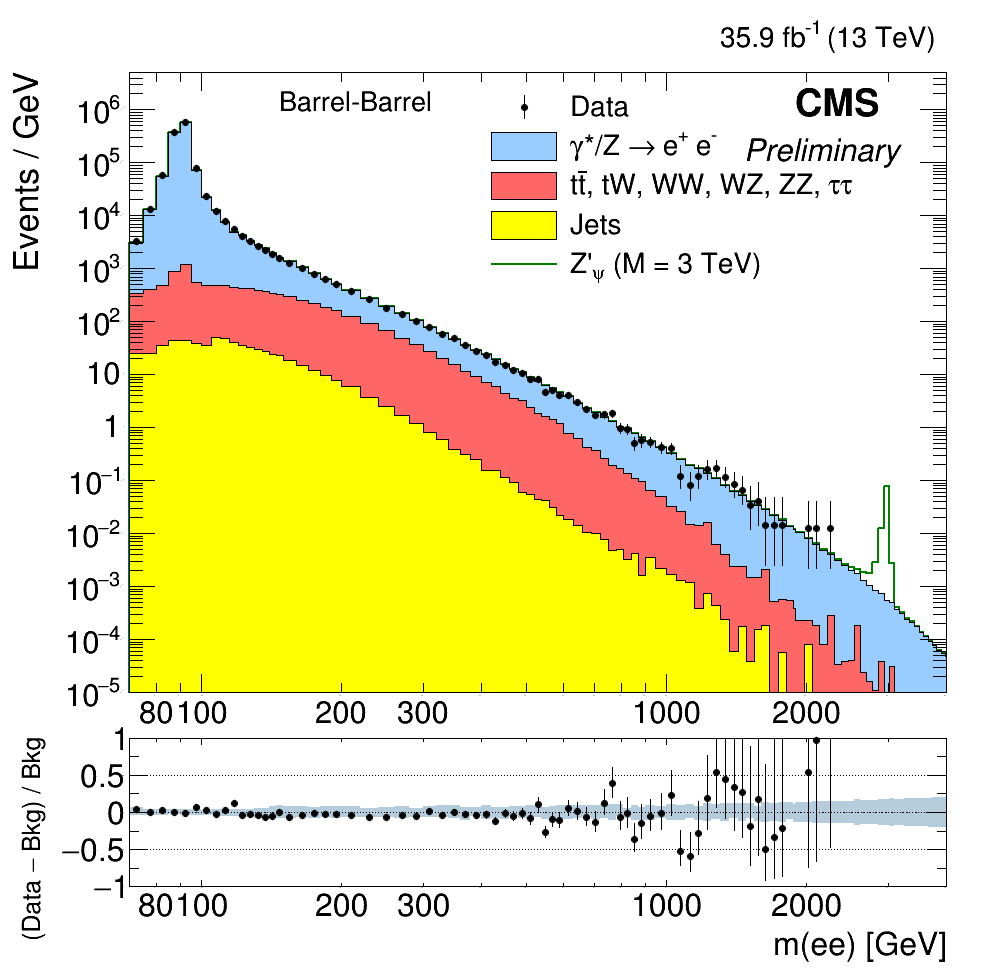
\includegraphics[width=0.47\textwidth]{figures/Zprime/2016/mass/massHistEBEB}
    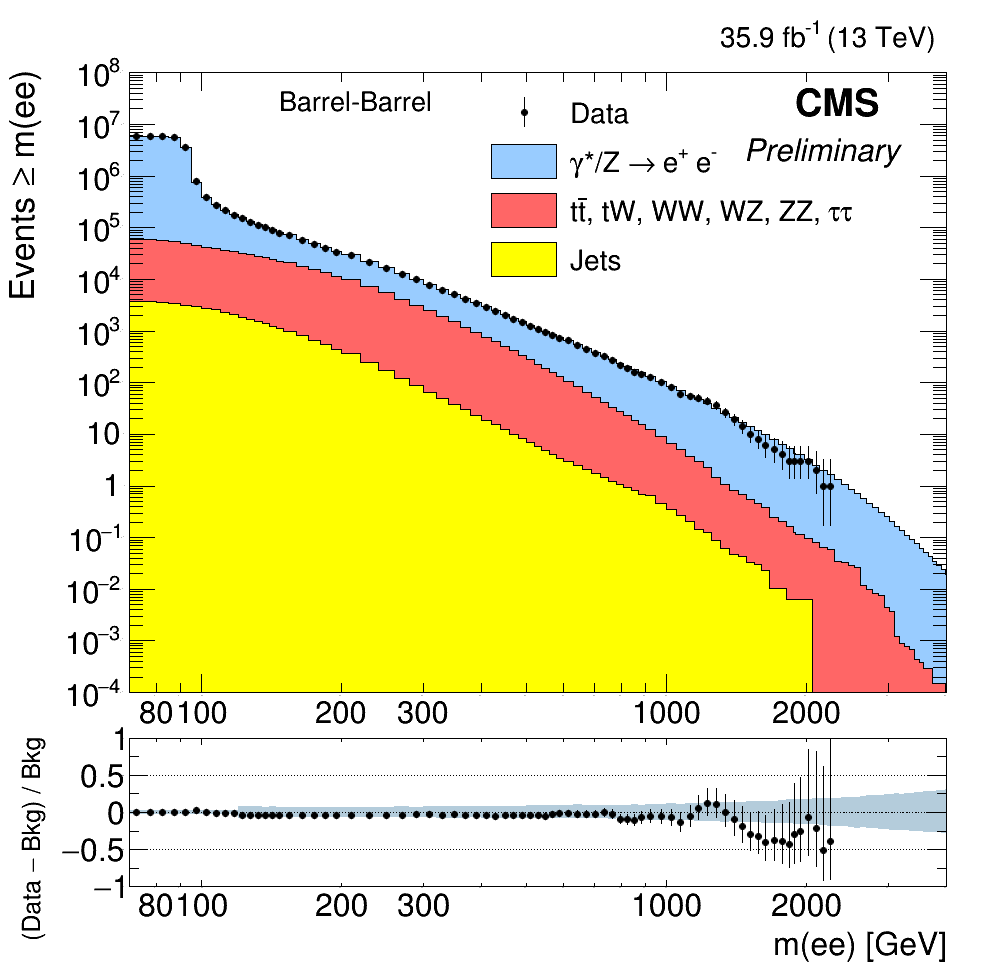
\includegraphics[width=0.47\textwidth]{figures/Zprime/2016/mass/cMassHistEBEB}
    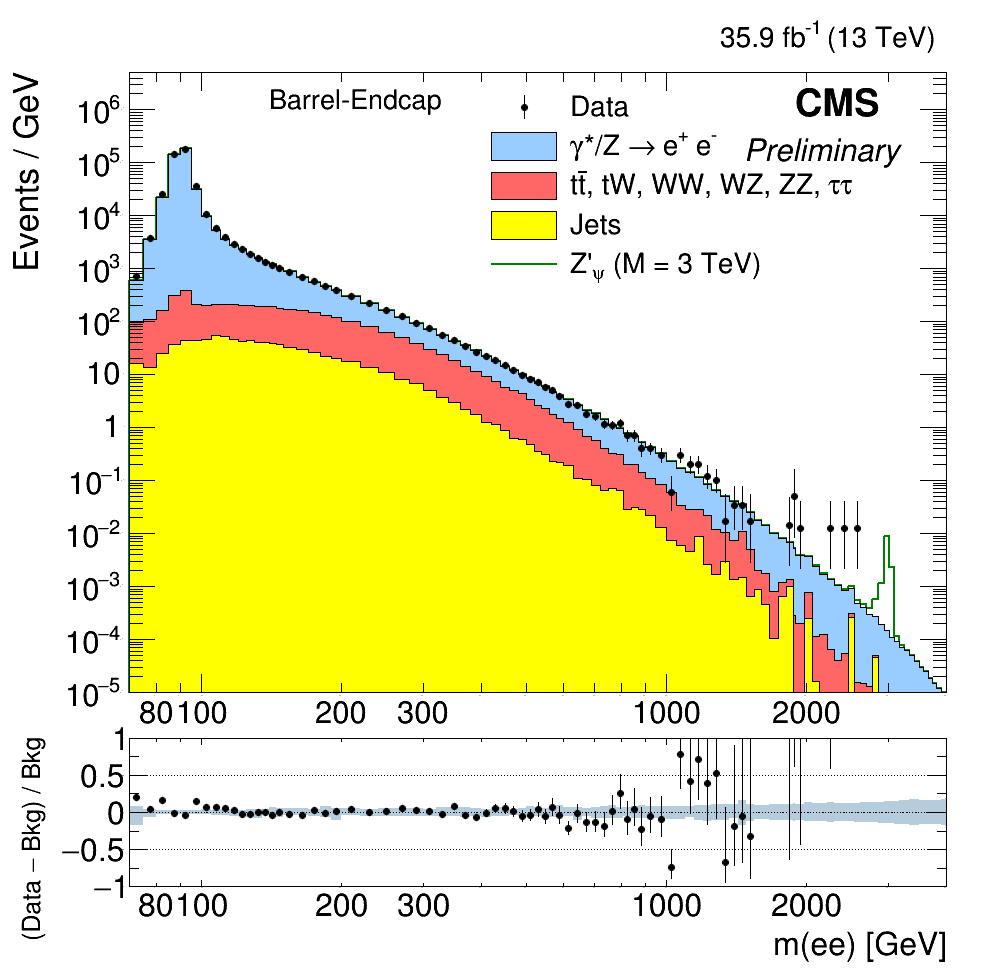
\includegraphics[width=0.47\textwidth]{figures/Zprime/2016/mass/massHistEBEE}
    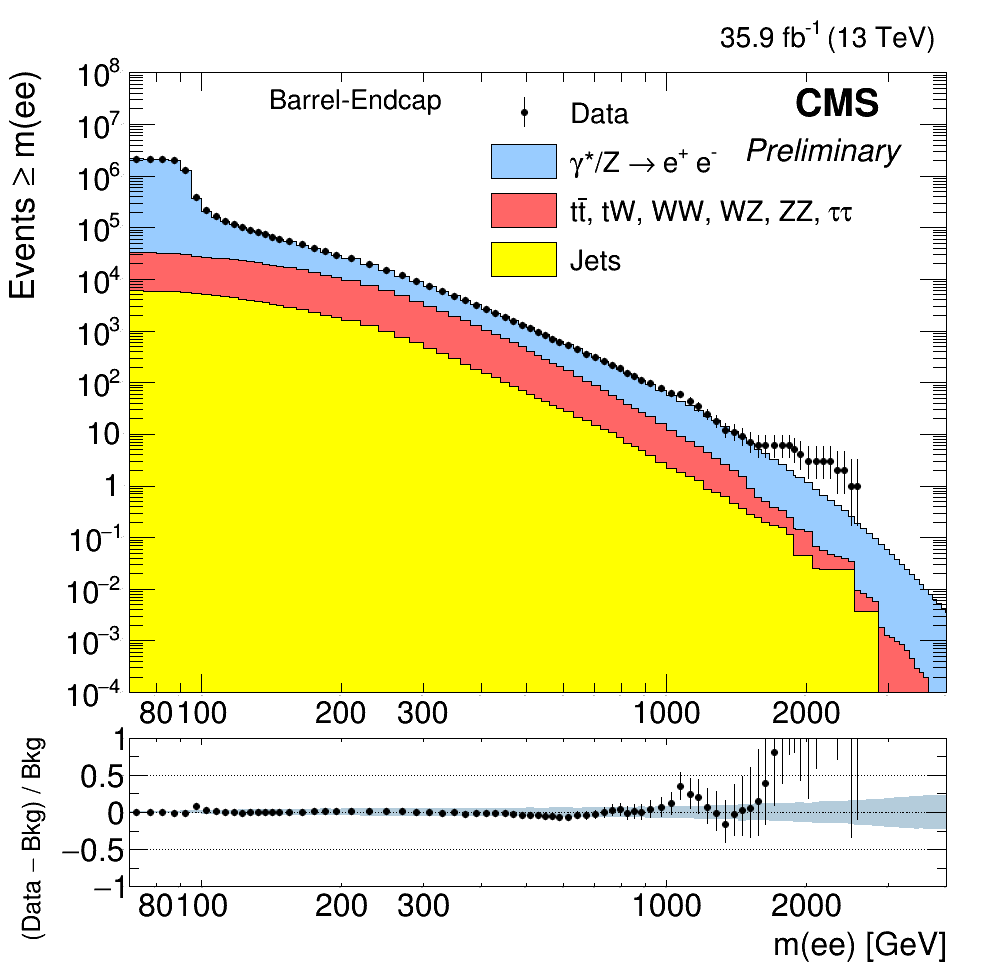
\includegraphics[width=0.47\textwidth]{figures/Zprime/2016/mass/cMassHistEBEE}
    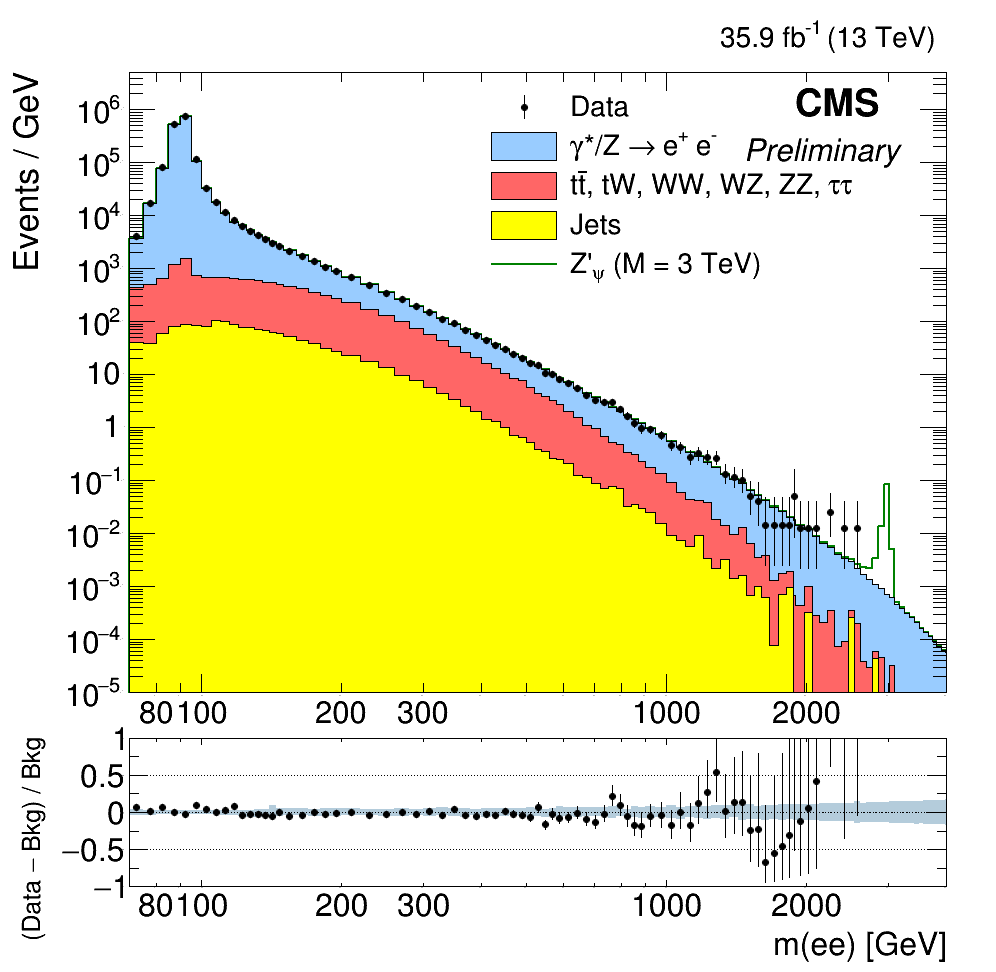
\includegraphics[width=0.47\textwidth]{figures/Zprime/2016/mass/massHist}
    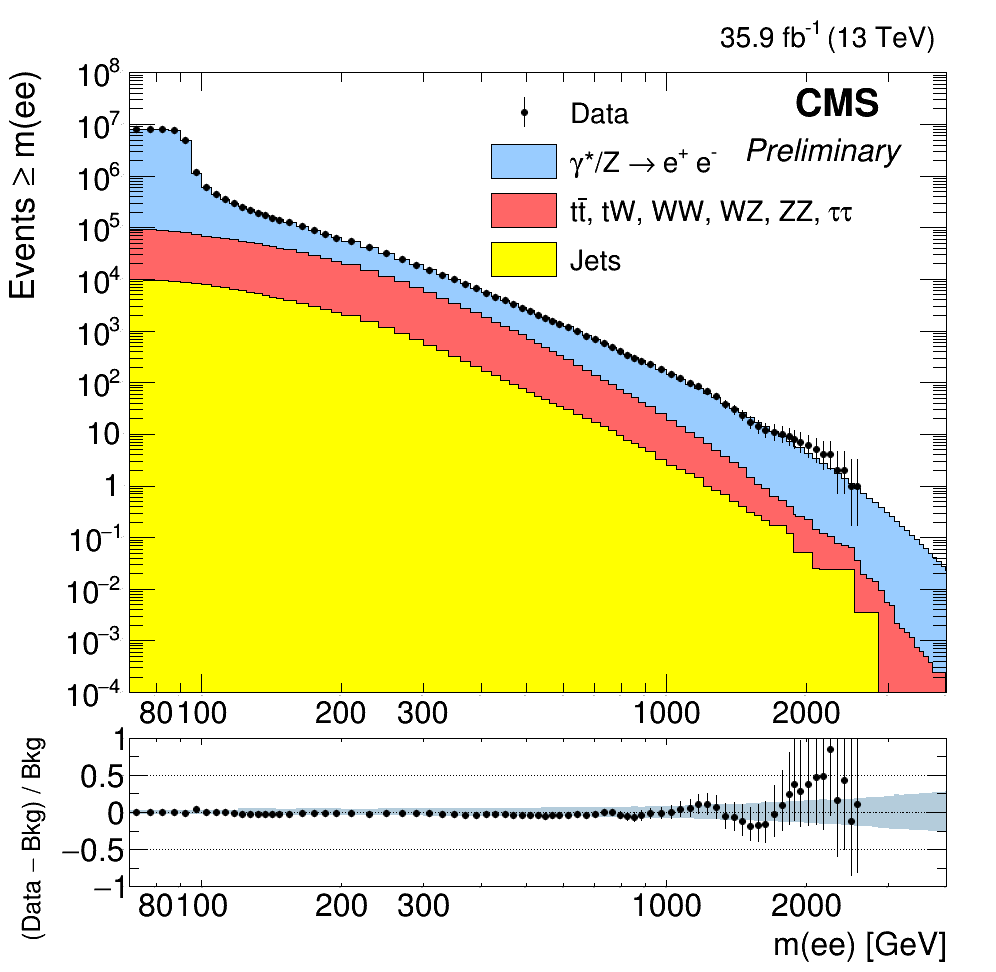
\includegraphics[width=0.47\textwidth]{figures/Zprime/2016/mass/cMassHist}
    \caption{The observed dielectron mass spectrum (left) and the integral of the measured dielectron mass spectrum (right) for barrel-barrel (top), barrel-endcap (middle) and sum of the barrel-barrel and the barrel-endcap (bottom) together with the predicted standard model backgrounds in 2016.}
    \label{mass_2016}
  \end{center}
\end{figure}

\begin{figure}
  \begin{center}
    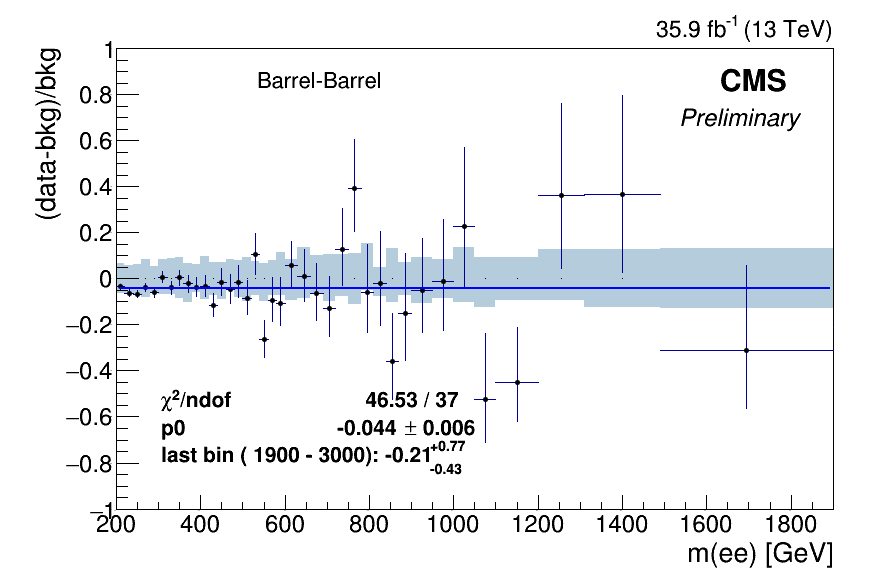
\includegraphics[width=0.47\textwidth]{figures/Zprime/2016/mass/SignalRegionHistEBEB_ratio}
    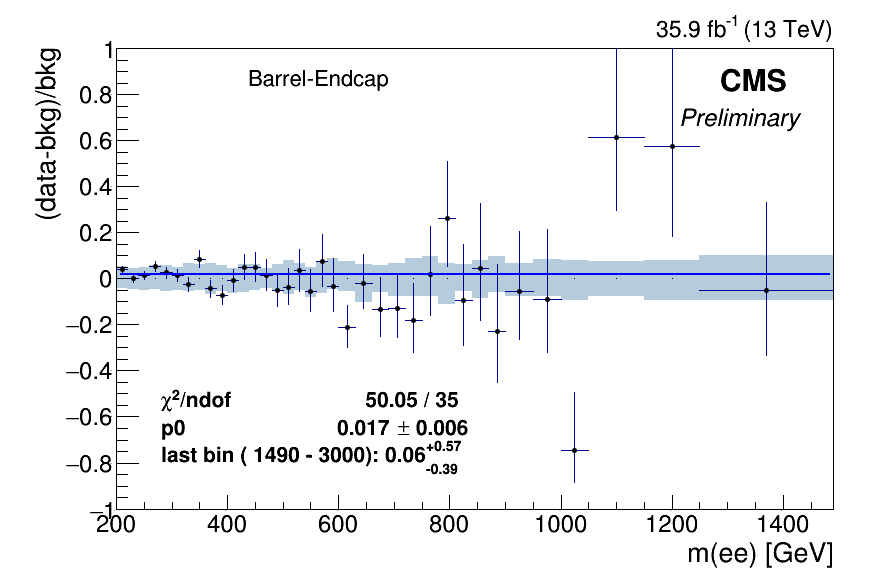
\includegraphics[width=0.47\textwidth]{figures/Zprime/2016/mass/SignalRegionHistEBEE_ratio}
    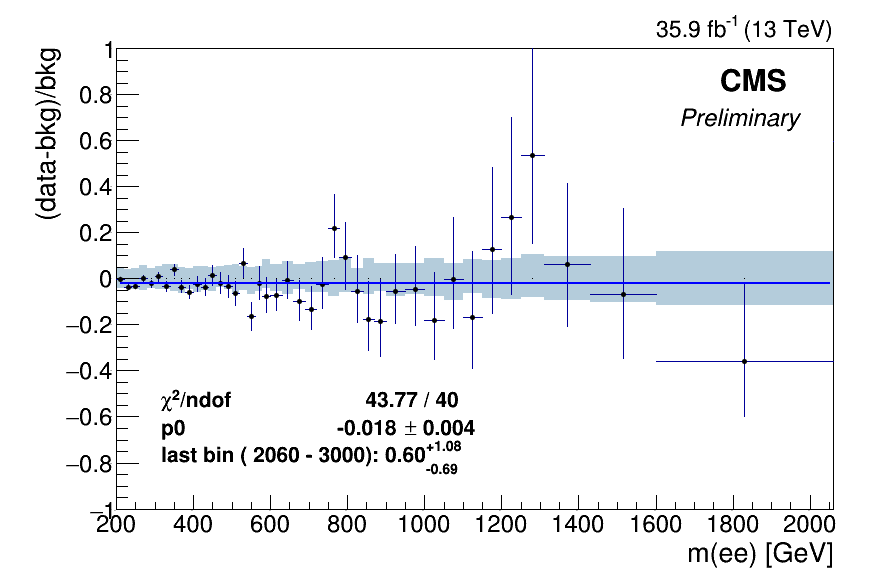
\includegraphics[width=0.47\textwidth]{figures/Zprime/2016/mass/SignalRegionHist_ratio}
    \caption{The ratio of observed dielectron mass spectrum in signal region for barrel-barrel (top left), barrel-endcap (top right) and sum of the barrel-barrel and the barrel-endcap together (bottom) in 2016.}
    \label{massratio_2016}
  \end{center}
\end{figure}

\begin{figure}[ht]
  \begin{center}
    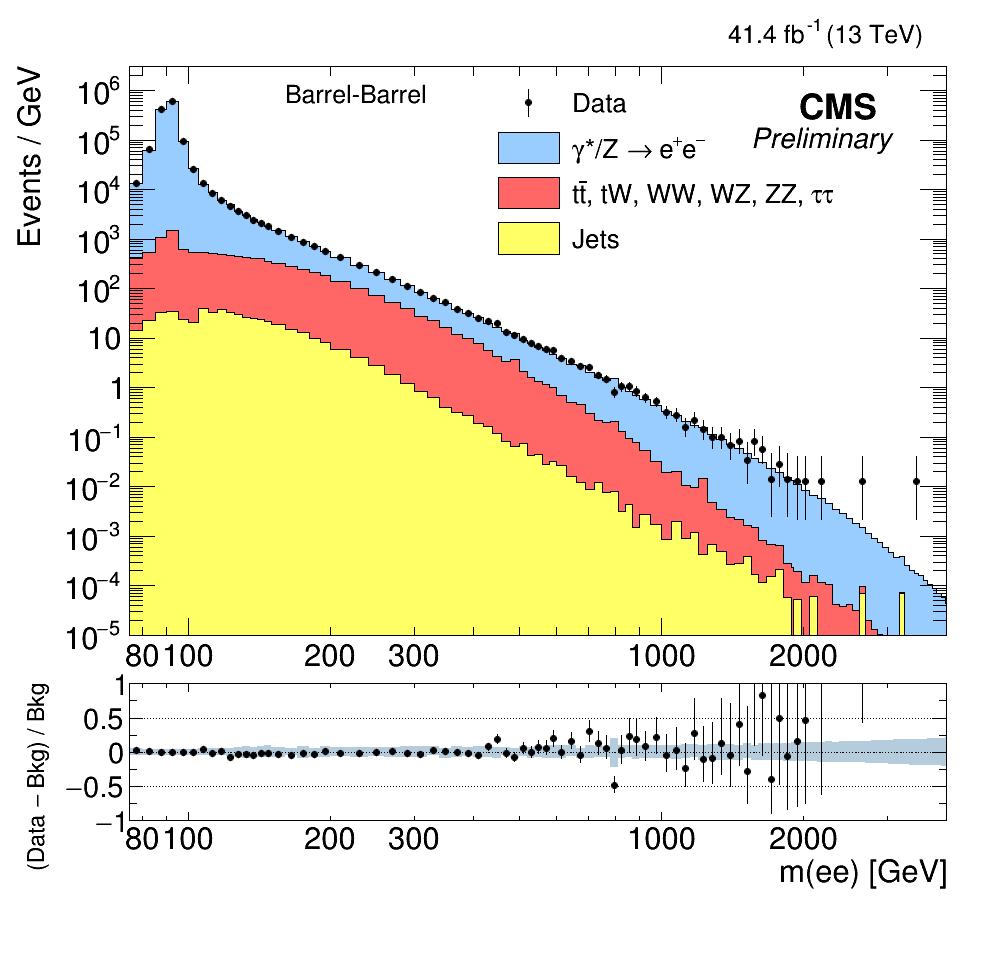
\includegraphics[width=0.47\textwidth]{figures/Zprime/2017/mass/massHistEBEB}
    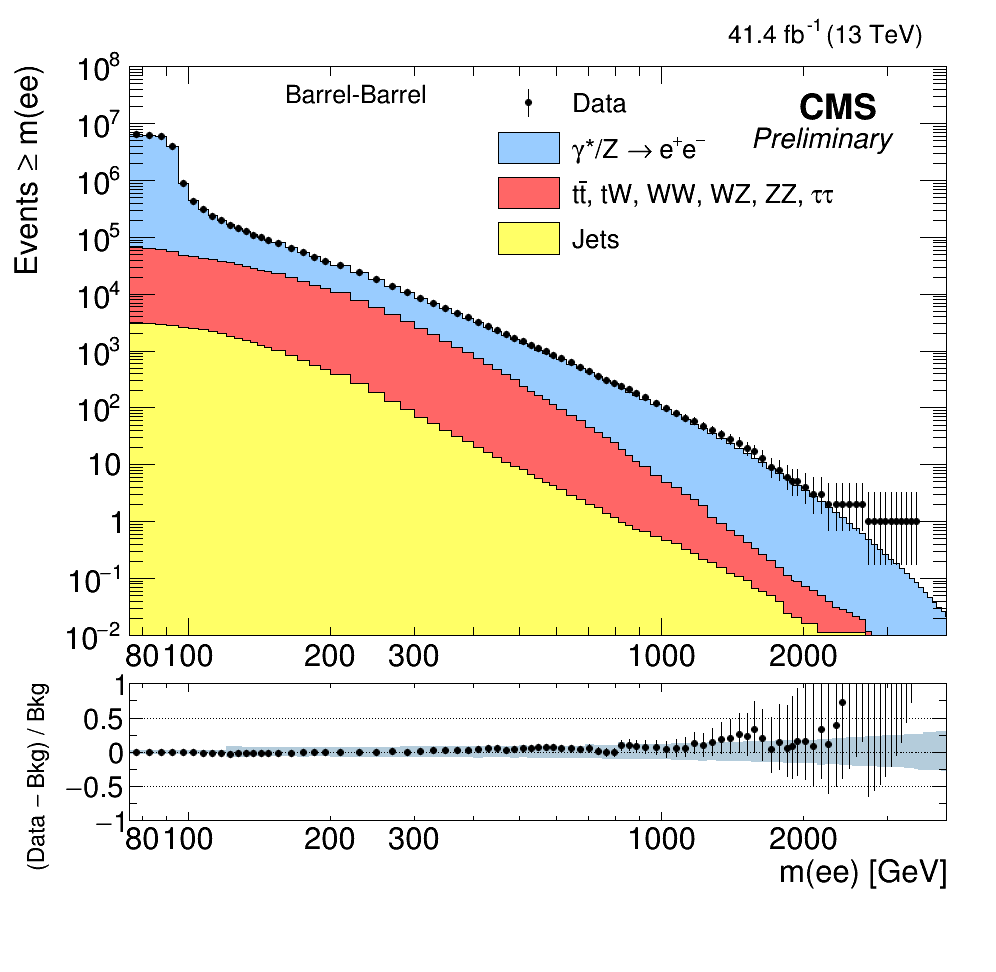
\includegraphics[width=0.47\textwidth]{figures/Zprime/2017/mass/cMassHistEBEB}
    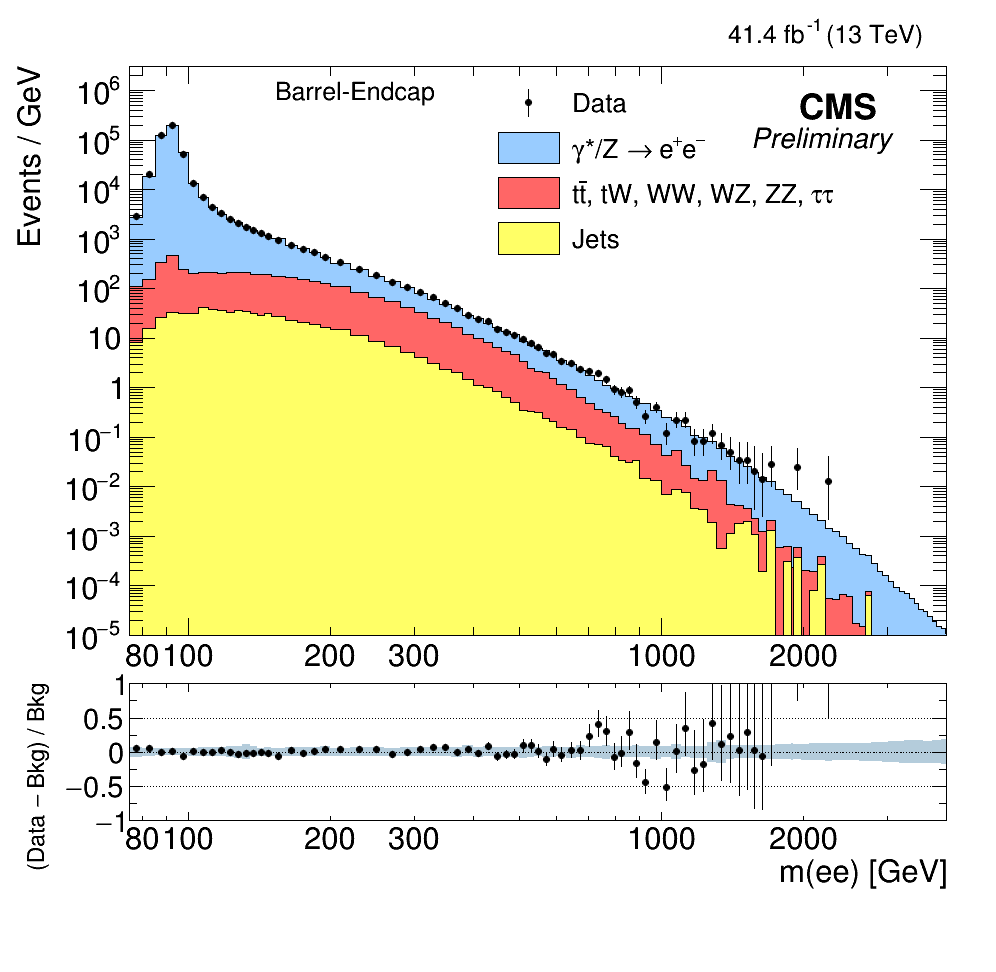
\includegraphics[width=0.47\textwidth]{figures/Zprime/2017/mass/massHistEBEE}
    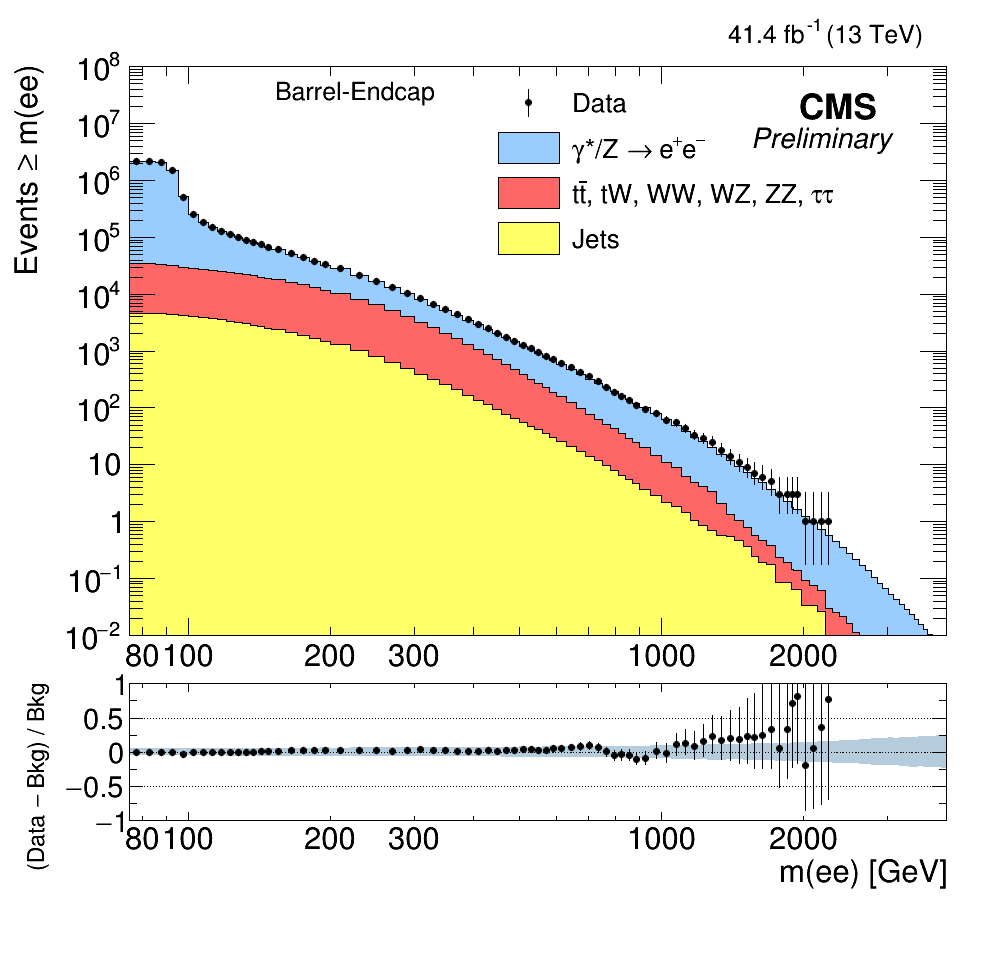
\includegraphics[width=0.47\textwidth]{figures/Zprime/2017/mass/cMassHistEBEE}
    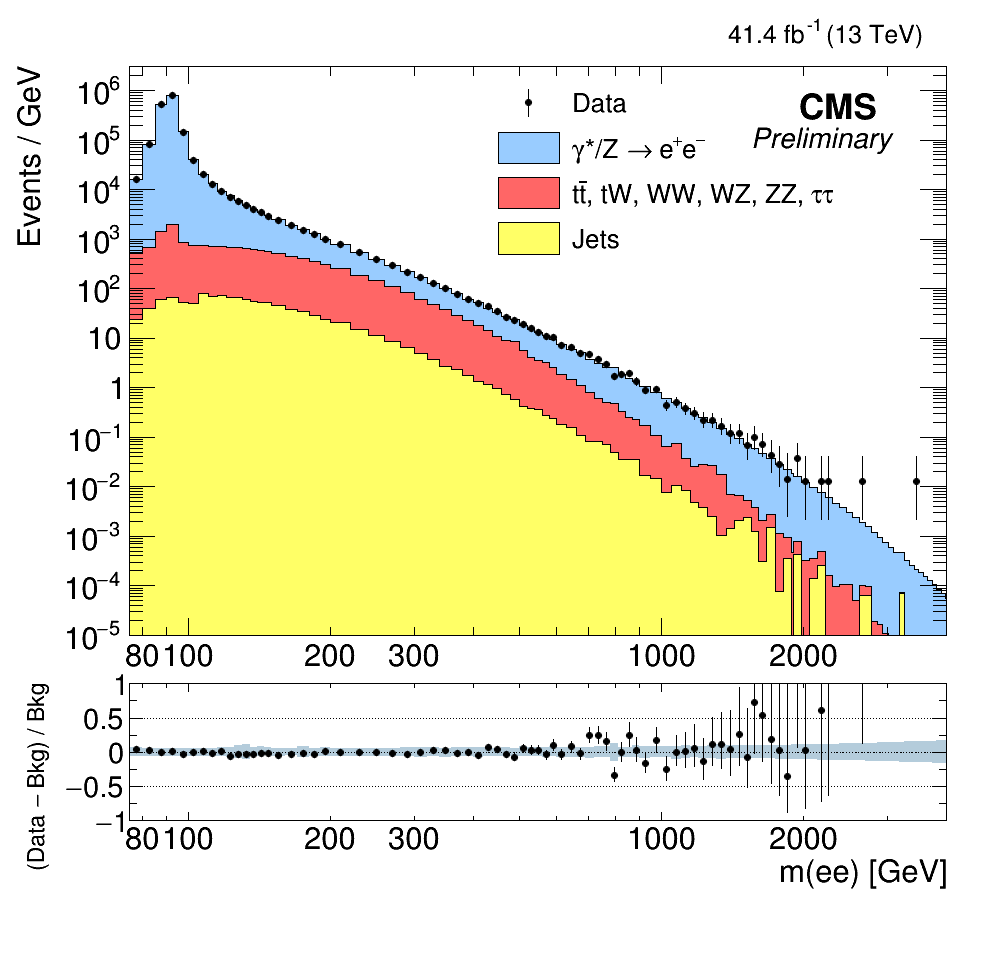
\includegraphics[width=0.47\textwidth]{figures/Zprime/2017/mass/massHist}
    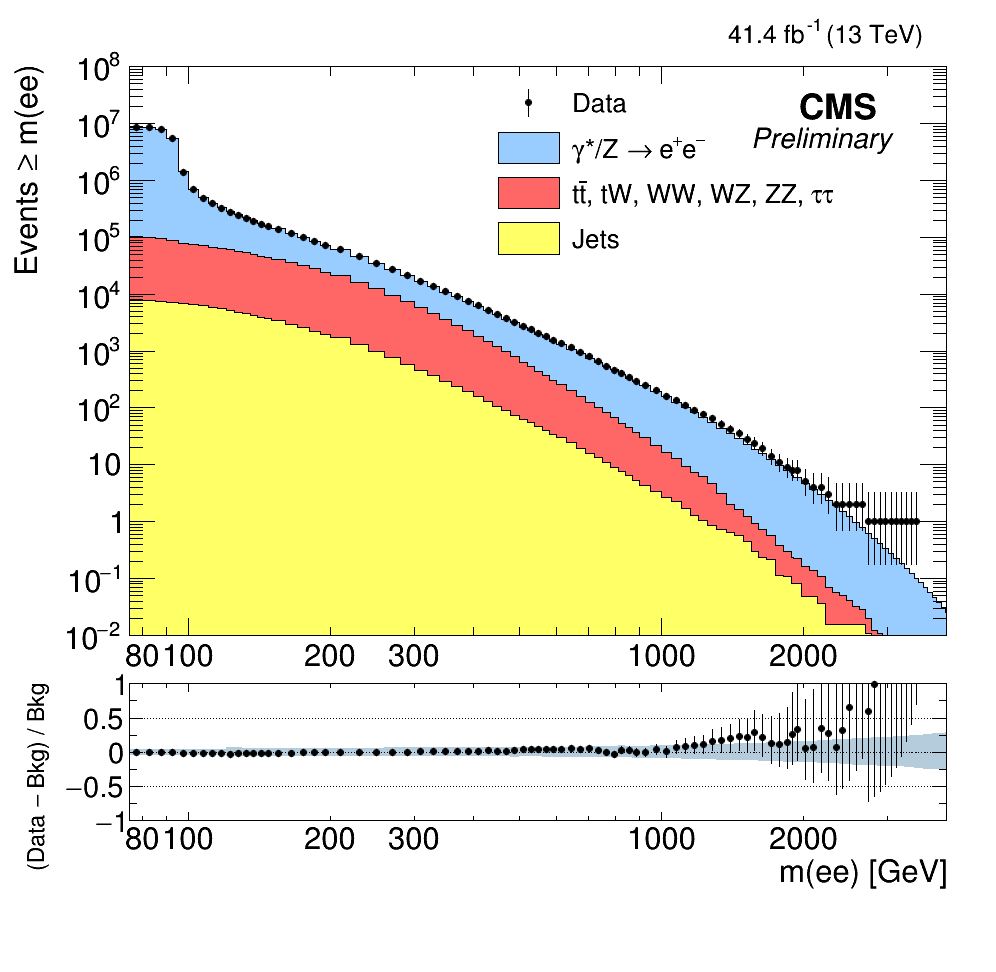
\includegraphics[width=0.47\textwidth]{figures/Zprime/2017/mass/cMassHist}
    \caption{The observed dielectron mass spectrum (left) and the integral of the measured dielectron mass spectrum (right) for barrel-barrel (top), barrel-endcap (middle) and sum of the barrel-barrel and the barrel-endcap (bottom) together with the predicted standard model backgrounds in 2017.}
    \label{mass_2017}
  \end{center}
\end{figure}



\begin{figure}
  \begin{center}
    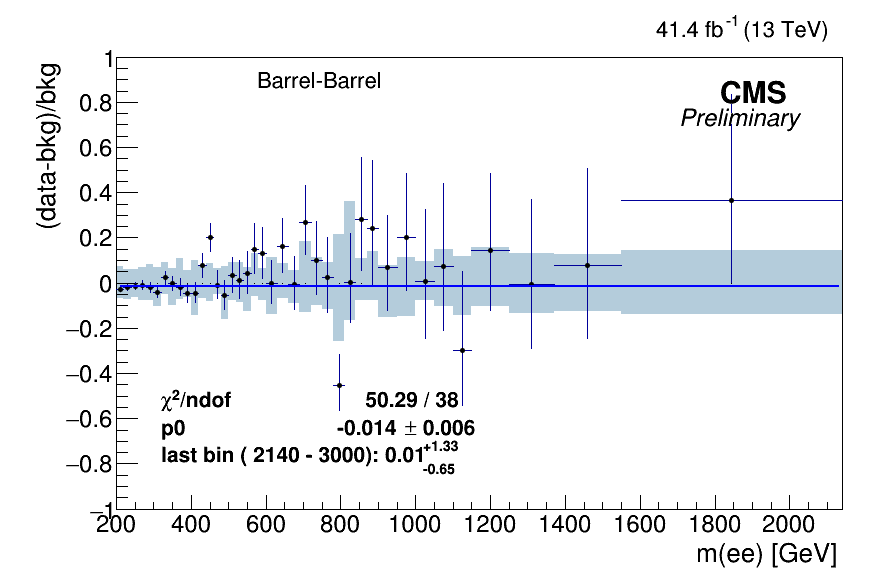
\includegraphics[width=0.47\textwidth]{figures/Zprime/2017/mass/SignalRegionHistEBEB}
    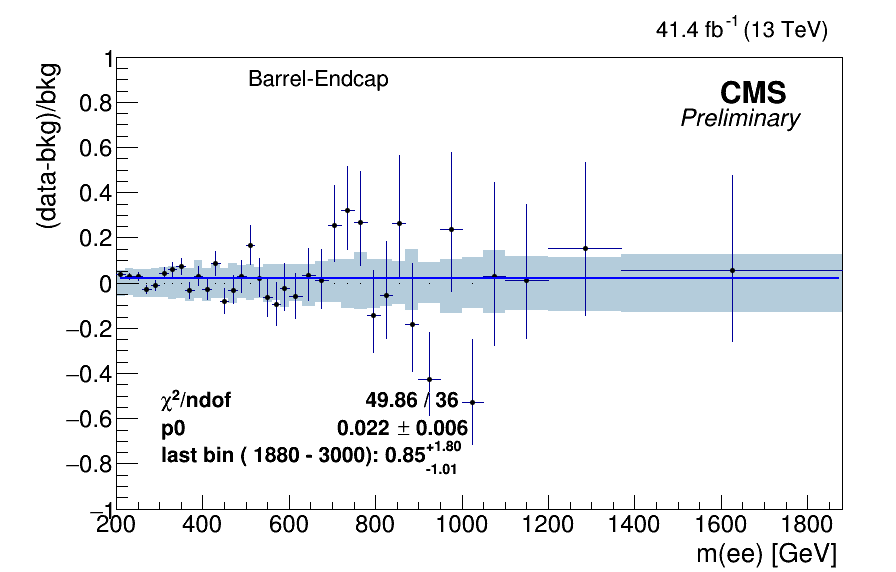
\includegraphics[width=0.47\textwidth]{figures/Zprime/2017/mass/SignalRegionHistEBEE}
    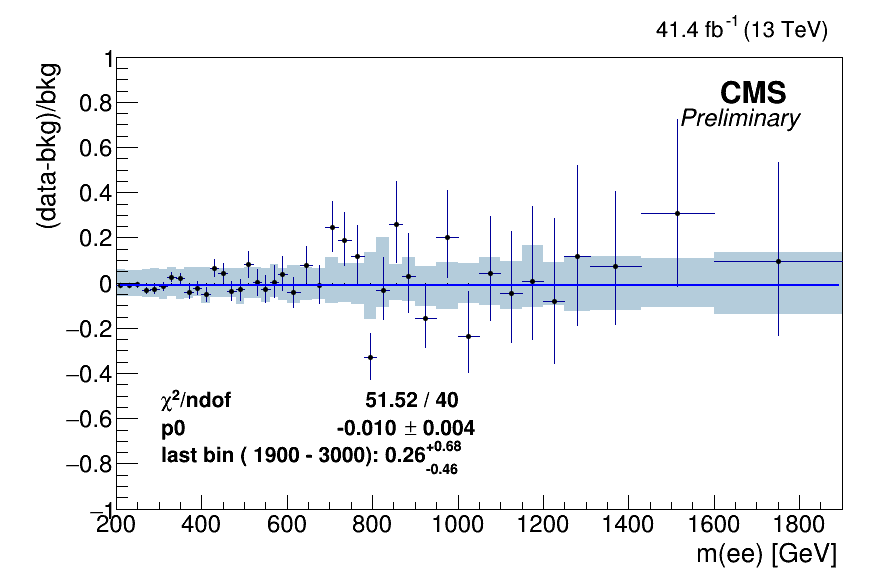
\includegraphics[width=0.47\textwidth]{figures/Zprime/2017/mass/SignalRegionHist}
    \caption{The ratio of observed dielectron mass spectrum in signal region for barrel-barrel (top left), barrel-endcap (top right) and sum of the barrel-barrel and the barrel-endcap together (bottom) in 2017.}
    \label{massratio_2017}
  \end{center}
\end{figure}



In Table \ref{data-MCn}, predicted SM background and observed data yields are shown as a function of dielectron invariant mass.

\begin{table}[htp]
\small
\caption{Predicted SM background and observed data yields as a function of dielectron invariant mass for Barrel-Barrel, Barrel-Endcap and Barrel-Barrel plus Barrel-Endcap. The uncertainty contains statistic uncertainty and systematic uncertainty}
\label{data-MCn}
\begin{center}
\scalebox{0.8}{
  \begin{tabular}{|l|l|l|l|l|l|l|}
    \hline
Year&Mass range    & data      & total bkg                 & $\gamma^*$/Z $\rightarrow$ ee    & $\ttbar$ and $\ttbar$-like bkg  & Jets\\ \hline \hline
\multirow{24}{*}{2016}&\multicolumn{6}{c|}{Barrel-Barrel} \\ \cline{2-7}
& 60    -- 120   & 5760346     & 5762889.7  $\pm$ 133911.3 & 5730973.8  $\pm$ 133096.7         & 29369.6    $\pm$ 1277.6    & 2546.3     $\pm$ 1273.2   \\
& 120   -- 400   & 146598      & 152496.1   $\pm$ 11452.7  & 120819.5   $\pm$ 10364.5          & 29824.2    $\pm$ 1572.3    & 1852.5     $\pm$ 926.2    \\
& 400   -- 600   & 2163        & 2295.3     $\pm$ 183.6    & 1636.5     $\pm$ 124.6            & 643.5      $\pm$ 63.2      & 15.4       $\pm$ 7.7      \\
& 600   -- 900   & 523         & 520.1      $\pm$ 51.1     & 425.9      $\pm$ 39.2             & 91.8       $\pm$ 13.3      & 2.4        $\pm$ 1.2      \\
& 900   -- 1300  & 100         & 107.9      $\pm$ 10.6     & 96.5       $\pm$ 9.4              & 10.9       $\pm$ 1.8       & 0.6        $\pm$ 0.3      \\
& 1300  -- 1800  & 24          & 21.5       $\pm$ 2.8      & 20.5       $\pm$ 2.6              & 0.9        $\pm$ 0.2       & 0.1        $\pm$ 0.0      \\
& 1800  -- 6000  & 3           & 5.4        $\pm$ 0.9      & 5.2        $\pm$ 0.9              & 0.2        $\pm$ 0.0       & 0.0        $\pm$ 0.0      \\ \cline{2-7}
&\multicolumn{6}{c|}{Barrel-Endcap} \\ \cline{2-7}
& 60    -- 120   & 2051759     & 2054401.1  $\pm$ 40405.8  & 2042472.6  $\pm$ 40296.8          & 9270.3     $\pm$ 345.6     & 2658.2     $\pm$ 1329.1   \\
& 120   -- 400   & 98503       & 99151.9    $\pm$ 4158.3   & 77350.1    $\pm$ 3306.5           & 17813.2    $\pm$ 728.6     & 3988.6     $\pm$ 1994.3   \\
& 400   -- 600   & 2134        & 2117.0     $\pm$ 112.6    & 1243.8     $\pm$ 58.0             & 751.3      $\pm$ 44.6      & 121.9      $\pm$ 61.0     \\
& 600   -- 900   & 420         & 463.3      $\pm$ 27.9     & 311.7      $\pm$ 18.5             & 128.3      $\pm$ 9.9       & 23.2       $\pm$ 11.6     \\
& 900   -- 1300  & 82          & 78.4       $\pm$ 5.9      & 59.2       $\pm$ 4.6              & 15.9       $\pm$ 1.6       & 3.3        $\pm$ 1.7      \\
& 1300  -- 1800  & 9           & 12.8       $\pm$ 1.2      & 10.3       $\pm$ 1.0              & 1.9        $\pm$ 0.4       & 0.6        $\pm$ 0.3      \\
& 1800  -- 6000  & 6           & 2.1        $\pm$ 0.3      & 1.8        $\pm$ 0.2              & 0.1        $\pm$ 0.0       & 0.1        $\pm$ 0.1      \\ \cline{2-7}
&\multicolumn{6}{c|}{Barrel-Barrel + Barrel-Endcap} \\ \cline{2-7}
& 60    -- 120   & 7812105     & 7817300.8  $\pm$ 166656.9 & 7773476.7  $\pm$ 165766.3         & 38627.6    $\pm$ 1524.1    & 5196.5     $\pm$ 2598.2   \\
& 120   -- 400   & 245101      & 252071.4   $\pm$ 12933.9  & 198526.1   $\pm$ 11326.7          & 47709.5    $\pm$ 2148.8    & 5835.8     $\pm$ 2917.9   \\
& 400   -- 600   & 4297        & 4424.5     $\pm$ 232.4    & 2887.1     $\pm$ 147.9            & 1400.2     $\pm$ 87.6      & 137.2      $\pm$ 68.6     \\
& 600   -- 900   & 943         & 985.9      $\pm$ 63.9     & 739.3      $\pm$ 48.7             & 221.0      $\pm$ 17.2      & 25.6       $\pm$ 12.8     \\
& 900   -- 1300  & 182         & 186.6      $\pm$ 13.5     & 155.9      $\pm$ 11.9             & 26.8       $\pm$ 2.3       & 3.9        $\pm$ 1.9      \\
& 1300  -- 1800  & 33          & 34.3       $\pm$ 3.4      & 30.9       $\pm$ 3.2              & 2.8        $\pm$ 0.5       & 0.6        $\pm$ 0.3      \\
& 1800  -- 6000  & 9           & 7.5        $\pm$ 1.1      & 7.0        $\pm$ 1.1              & 0.3        $\pm$ 0.0       & 0.1        $\pm$ 0.1      \\  \cline{2-7} \hline \hline
\multirow{24}{*}{2017}& \multicolumn{6}{c|}{Barrel-Barrel} \\ \cline{2-7}
& 60    -- 120   & 6190697        & 6194808.2  $\pm$ 178177.2   & 6156571.2  $\pm$ 177324.0         & 34116.3    $\pm$ 1921.1           & 4120.7      \\
& 120   -- 400   & 162005         & 167925.2   $\pm$ 13932.9    & 132981.8   $\pm$ 12618.8          & 33128.5    $\pm$ 2365.8           & 1815.0      \\
& 400   -- 600   & 2503           & 2404.7     $\pm$ 215.9      & 1782.7     $\pm$ 144.5            & 605.2      $\pm$ 79.6             & 16.8        \\
& 600   -- 900   & 588            & 560.2      $\pm$ 51.5       & 478.6      $\pm$ 44.9             & 78.7       $\pm$ 15.6             & 3.0         \\
& 900   -- 1300  & 118            & 113.4      $\pm$ 13.1       & 105.1      $\pm$ 11.4             & 7.8        $\pm$ 2.8              & 0.5         \\
& 1300  -- 1800  & 28             & 23.1       $\pm$ 3.0        & 23.0       $\pm$ 3.0              & 0.0        $\pm$ 0.0              & 0.1         \\
& 1800  -- 6000  & 7              & 5.7        $\pm$ 1.0        & 5.7        $\pm$ 1.0              & 0.0        $\pm$ 0.0              & 0.0         \\  \cline{2-7}
&\multicolumn{6}{c|}{Barrel-Endcap} \\ \cline{2-7}
& 60    -- 120   & 2096490        & 2098260.5  $\pm$ 96902.6    & 2086010.3  $\pm$ 96566.8          & 10473.3    $\pm$ 675.3            & 1777.0     \\
& 120   -- 400   & 109771         & 110357.8   $\pm$ 6227.6     & 87277.3    $\pm$ 5107.0           & 19860.0    $\pm$ 1450.6           & 3220.6     \\
& 400   -- 600   & 2365           & 2364.5     $\pm$ 164.6      & 1442.8     $\pm$ 99.9             & 810.5      $\pm$ 68.3             & 111.3      \\
& 600   -- 900   & 518            & 488.3      $\pm$ 37.9       & 341.8      $\pm$ 26.5             & 124.1      $\pm$ 13.9             & 22.4       \\
& 900   -- 1300  & 75             & 86.5       $\pm$ 7.7        & 69.5       $\pm$ 6.3              & 14.0       $\pm$ 2.7              & 3.0        \\
& 1300  -- 1800  & 16             & 14.2       $\pm$ 1.7        & 11.7       $\pm$ 1.3              & 2.0        $\pm$ 1.0              & 0.6        \\
& 1800  -- 6000  & 3              & 2.2        $\pm$ 0.3        & 2.1        $\pm$ 0.3              & 0.0        $\pm$ 0.0              & 0.1        \\  \cline{2-7}
&\multicolumn{6}{c|}{Barrel-Barrel + Barrel-Endcap} \\ \cline{2-7}
& 60    -- 120   & 8287187        & 8290233.1  $\pm$ 369104.3   & 8242650.8  $\pm$ 364680.2         & 44535.5    $\pm$ 2834.7           & 3046.7    \\
& 120   -- 400   & 271776         & 280802.3   $\pm$ 18298.7    & 222376.6   $\pm$ 15710.7          & 53411.9    $\pm$ 3976.3           & 5013.9    \\
& 400   -- 600   & 4868           & 4841.2     $\pm$ 329.4      & 3267.6     $\pm$ 216.8            & 1446.0     $\pm$ 128.0            & 127.6     \\
& 600   -- 900   & 1106           & 1062.0     $\pm$ 77.4       & 829.4      $\pm$ 63.0             & 207.4      $\pm$ 22.6             & 25.3      \\
& 900   -- 1300  & 193            & 201.3      $\pm$ 18.0       & 176.2      $\pm$ 16.0             & 21.6       $\pm$ 3.9              & 3.5       \\
& 1300  -- 1800  & 44             & 37.6       $\pm$ 4.2        & 34.8       $\pm$ 4.0              & 2.1        $\pm$ 1.1              & 0.7       \\
& 1800  -- 6000  & 10             & 7.9        $\pm$ 1.2        & 7.8        $\pm$ 1.2              & 0.0        $\pm$ 0.0              & 0.1       \\  \hline

\end{tabular}}
\end{center}
\end{table}




In Table \ref{systematic_effect}, the relative effect of each systematic uncertainty is shown as a function of dielectron invariant mass.

\begin{table}[htp]
\small
\caption{The relative effect of each systematic uncertainty as a function of dielectron invariant mass.}
\label{systematic_effect}
\begin{center}
\scalebox{0.8}{
\begin{tabular}{|l|l|l|l|l|l|l|l|l|}
\hline
Year&Uncertainty                 & 60-120         & 120-400        & 400-600        & 600-900       & 900-1300       & 1300-1800      & 1800-6000  \\\hline
\multirow{14}{*}{2016}&normalization\_scale\_up    & 0.998\%        & 0.972\%        & 0.966\%        &0.971\%        & 0.977\%        & 0.980\%        & 0.982\%    \\\cline{2-9}
&normalization\_scale\_down  & 0.998\%        & 0.972\%        & 0.966\%        &0.971\%        & 0.977\%        & 0.980\%        & 0.982\%    \\\cline{2-9}
&pdf\_scale\_up              & 0.147\%        & 0.165\%        & 1.122\%        &2.215\%        & 3.753\%        & 6.279\%        & 10.351\%   \\\cline{2-9}
&pdf\_scale\_down            & 0.096\%        & 0.025\%        & 1.000\%        &1.774\%        & 3.769\%        & 6.397\%        & 9.928\%    \\\cline{2-9}
&energy\_scale\_up           & 0.201\%        & 4.473\%        & 4.147\%        &4.925\%        & 4.830\%        & 6.523\%        & 8.699\%    \\\cline{2-9}
&energy\_scale\_down         & 0.095\%        & 4.325\%        & 3.930\%        &3.942\%        & 5.073\%        & 5.614\%        & 6.873\%    \\\cline{2-9}
&PU\_scale\_up               & 0.472\%        & 0.446\%        & 0.405\%        &0.827\%        & 0.323\%        & 0.050\%        & 0.729\%    \\\cline{2-9}
&PU\_scale\_down             & 0.424\%        & 0.262\%        & 0.353\%        &0.264\%        & 0.394\%        & 0.367\%        & 0.349\%    \\\cline{2-9}
&bgk\_scale\_up              & 0.036\%        & 1.334\%        & 1.870\%        &1.460\%        & 1.092\%        & 0.958\%        & 0.888\%    \\\cline{2-9}
&bgk\_scale\_down            & 0.036\%        & 1.334\%        & 1.870\%        &1.460\%        & 1.092\%        & 0.958\%        & 0.888\%    \\\cline{2-9}
&SF\_scale\_up               & 1.797\%        & 1.778\%        & 2.078\%        &2.893\%        & 3.065\%        & 3.590\%        & 4.949\%    \\\cline{2-9}
&SF\_scale\_down             & 1.711\%        & 1.510\%        & 1.991\%        &2.144\%        & 3.072\%        & 3.836\%        & 4.355\%    \\\cline{2-9}
&total\_scale\_up            & 2.124\%        & 5.111\%        & 5.231\%        &6.426\%        & 7.004\%        & 9.836\%        & 14.477\%   \\\cline{2-9}
&total\_scale\_down          & 2.031\%        & 4.877\%        & 4.996\%        &5.141\%        & 7.188\%        & 9.443\%        & 12.909\%   \\\hline \hline
\multirow{14}{*}{2017}&normalization\_scale\_up    & 4.033\%        & 3.900\%        & 3.882\%        & 3.895\%        & 3.922\%        & 3.922\%        & 3.937\%        \\\cline{2-9}
&normalization\_scale\_down  & 3.992\%        & 3.900\%        & 3.882\%        & 3.895\%        & 3.922\%        & 3.922\%        & 3.937\%        \\\cline{2-9}
&pdf\_scale\_up              & 0.114\%        & 0.125\%        & 1.021\%        & 2.102\%        & 3.941\%        & 6.456\%        & 10.549\%       \\\cline{2-9}
&pdf\_scale\_down            & 0.114\%        & 0.125\%        & 1.021\%        & 2.102\%        & 3.941\%        & 6.456\%        & 10.549\%       \\\cline{2-9}
&energy\_scale\_up           & 0.217\%        & 4.312\%        & 4.009\%        & 4.562\%        & 4.382\%        & 5.875\%        & 8.415\%        \\\cline{2-9}
&energy\_scale\_down         & 0.143\%        & 4.660\%        & 4.312\%        & 4.144\%        & 5.083\%        & 5.335\%        & 7.396\%        \\\cline{2-9}
&PU\_scale\_up               & 0.446\%        & 0.315\%        & 0.215\%        & 0.510\%        & 0.344\%        & 0.000\%        & 0.414\%        \\\cline{2-9}
&PU\_scale\_down             & 0.480\%        & 0.338\%        & 0.247\%        & 0.427\%        & 0.283\%        & 0.096\%        & 0.422\%        \\\cline{2-9}
&bkg\_scale\_up              & 0.029\%        & 1.391\%        & 2.036\%        & 1.491\%        & 0.959\%        & 0.952\%        & 0.773\%        \\\cline{2-9}
&bkg\_scale\_down            & 0.029\%        & 1.391\%        & 2.036\%        & 1.491\%        & 0.959\%        & 0.952\%        & 0.773\%        \\\cline{2-9}
&SF\_scale\_up               & 1.805\%        & 1.515\%        & 1.670\%        & 2.327\%        & 3.477\%        & 4.648\%        & 5.198\%        \\\cline{2-9}
&SF\_scale\_down             & 1.806\%        & 1.798\%        & 2.627\%        & 3.422\%        & 4.391\%        & 4.872\%        & 5.162\%        \\\cline{2-9}
&total\_scale\_up            & 4.448\%        & 6.176\%        & 6.258\%        & 6.950\%        & 7.953\%        & 10.681\%        & 15.012\%      \\\cline{2-9}
&total\_scale\_down          & 4.412\%        & 6.498\%        & 6.768\%        & 7.133\%        & 8.776\%        & 10.496\%        & 14.453\%      \\\hline

\end{tabular}}
\end{center}
\end{table}




\subsection{Complementary plot}
In addition to the invariant mass plot, the distributions of the following variables are shown in figures \ref{fig:complementary_2016} (\ref{fig:complementary_2017}) for 2016 (2017).
\begin{itemize}
  \item invariant mass of the selected electron pair in Z peak region for different catagories
  \item $E_{T}$, $\eta$ and $\phi$ of leading electron and sub-leading electron for $M_{ee}>200$ GeV
  \item $\Delta R$ and $\Delta\phi$ between selected electrons for $M_{ee}>200$ GeV
  \item $P_{T}$ of the reconstructed Z for $M_{ee}>200$ GeV
\end{itemize}



\begin{figure}[ht]
  \begin{center}
    \begin{tabular}{ccc}
      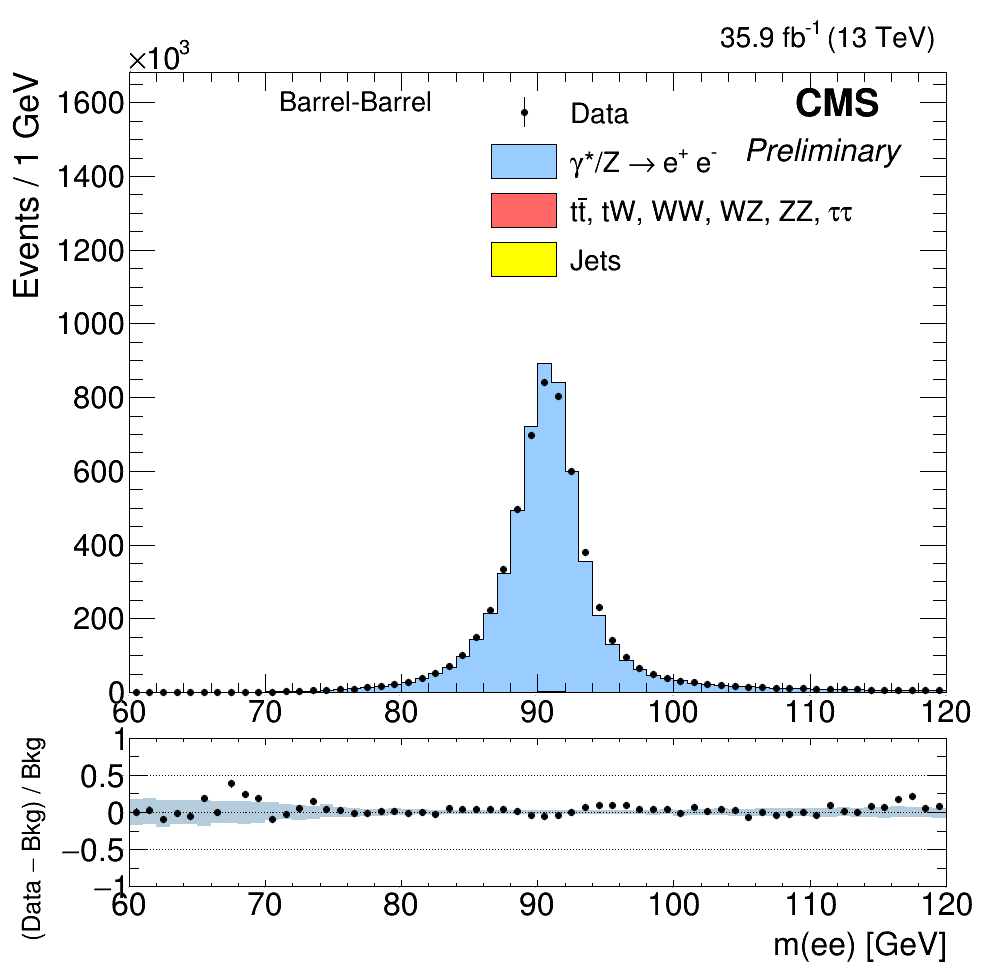
\includegraphics[width=0.32\textwidth]{figures/Zprime/2016/complementary/h_mee_Zpeak_BB.png}&
      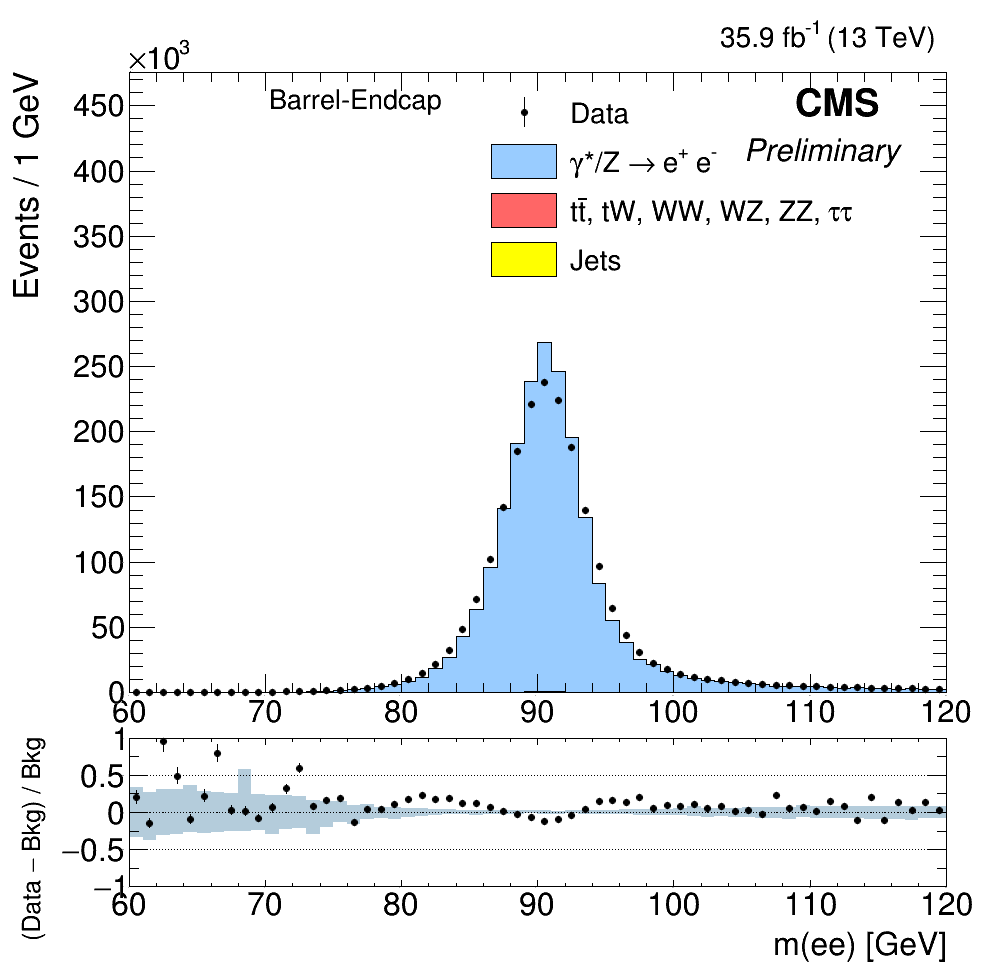
\includegraphics[width=0.32\textwidth]{figures/Zprime/2016/complementary/h_mee_Zpeak_BE.png}&
      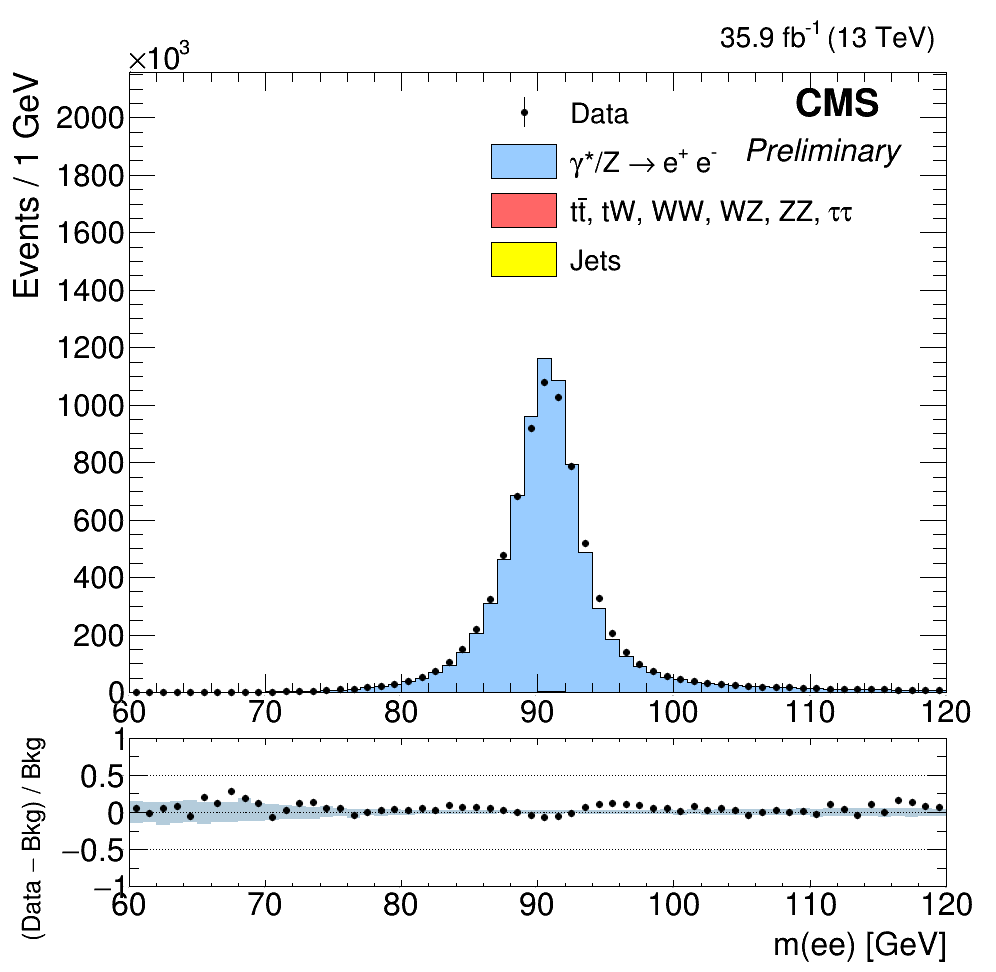
\includegraphics[width=0.32\textwidth]{figures/Zprime/2016/complementary/h_mee_Zpeak.png}\\
      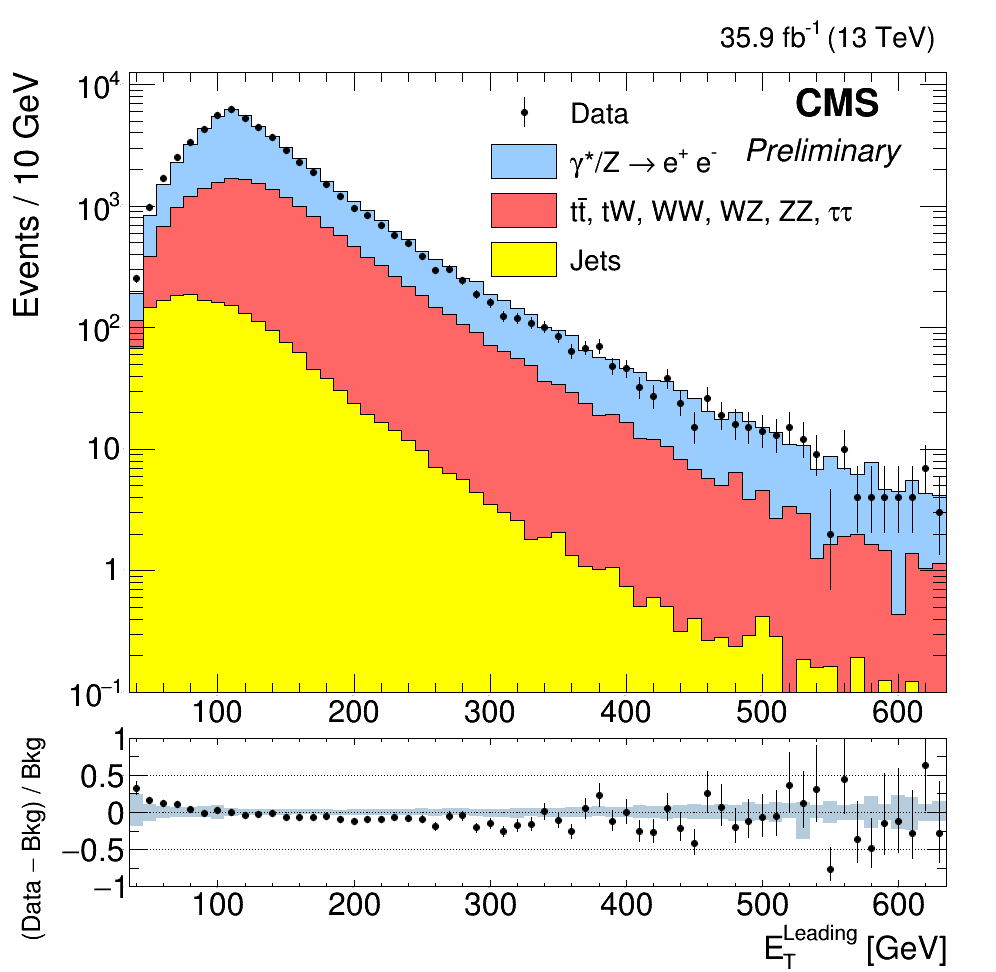
\includegraphics[width=0.32\textwidth]{figures/Zprime/2016/complementary/h_led_Et.png}&
      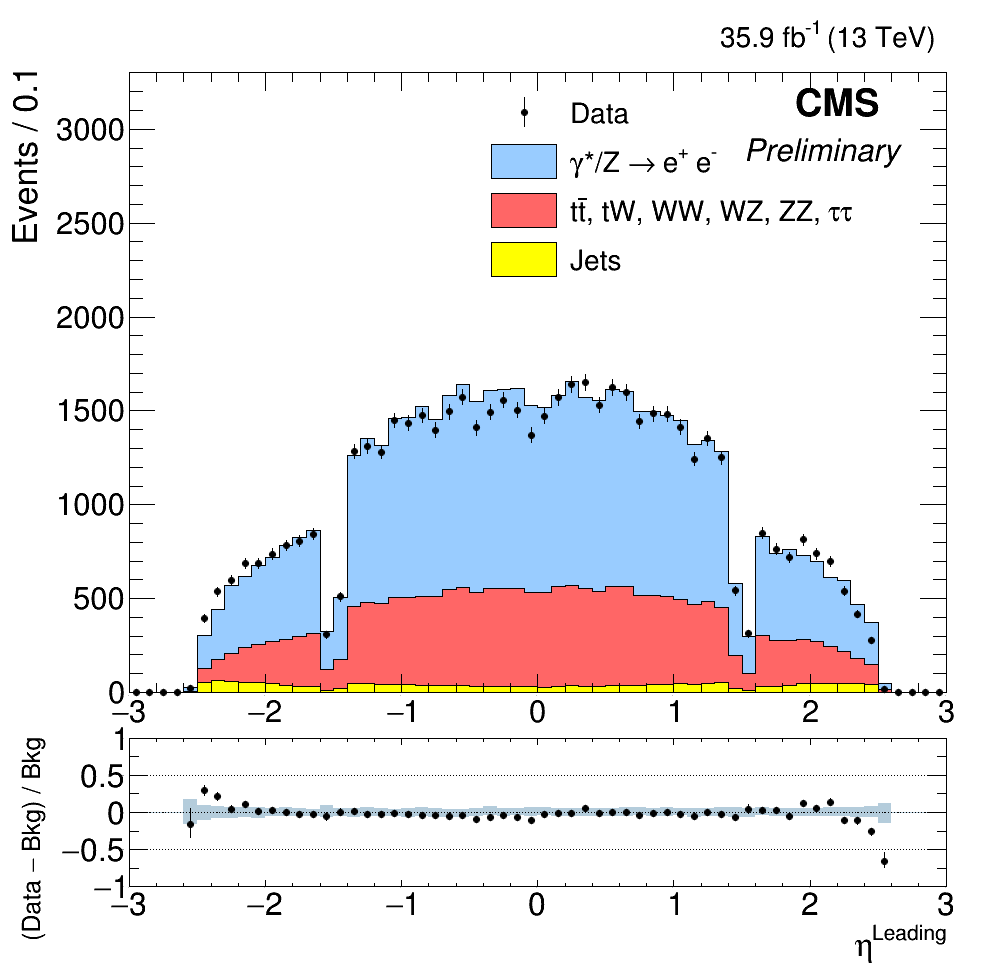
\includegraphics[width=0.32\textwidth]{figures/Zprime/2016/complementary/h_led_eta.png}&
      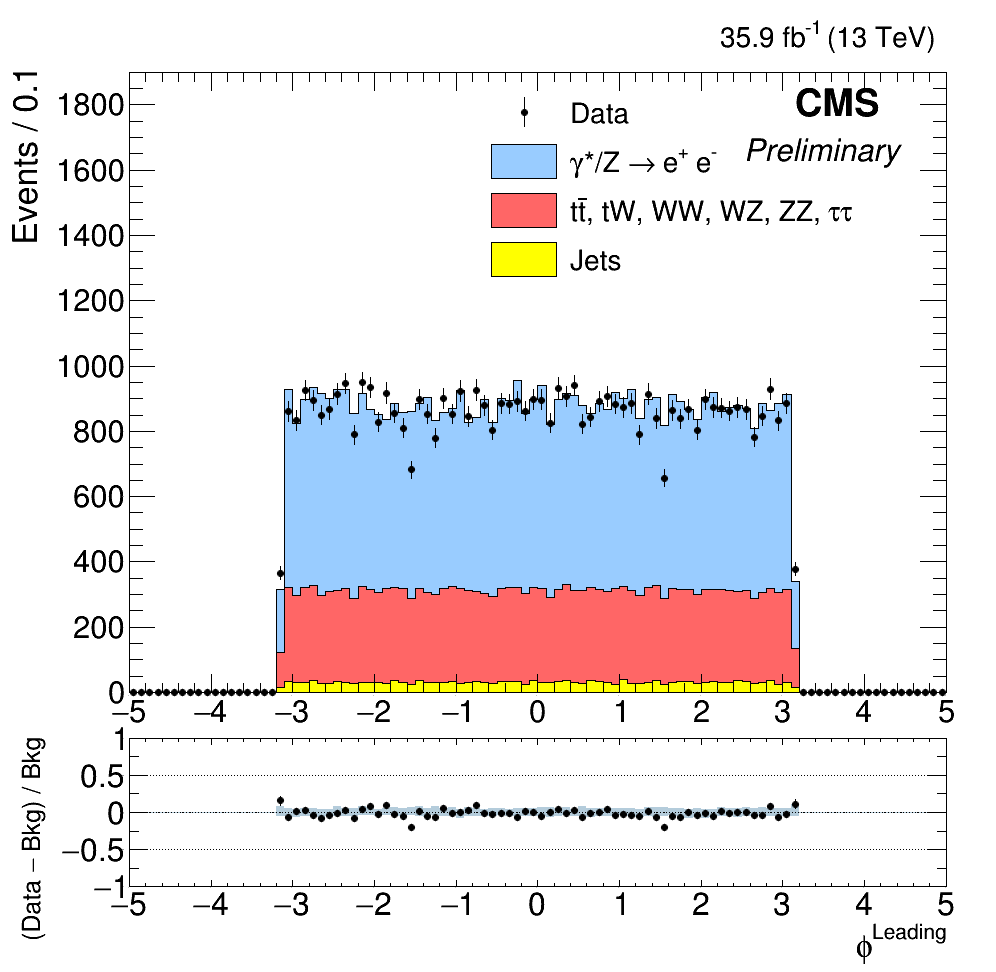
\includegraphics[width=0.32\textwidth]{figures/Zprime/2016/complementary/h_led_phi.png}\\
      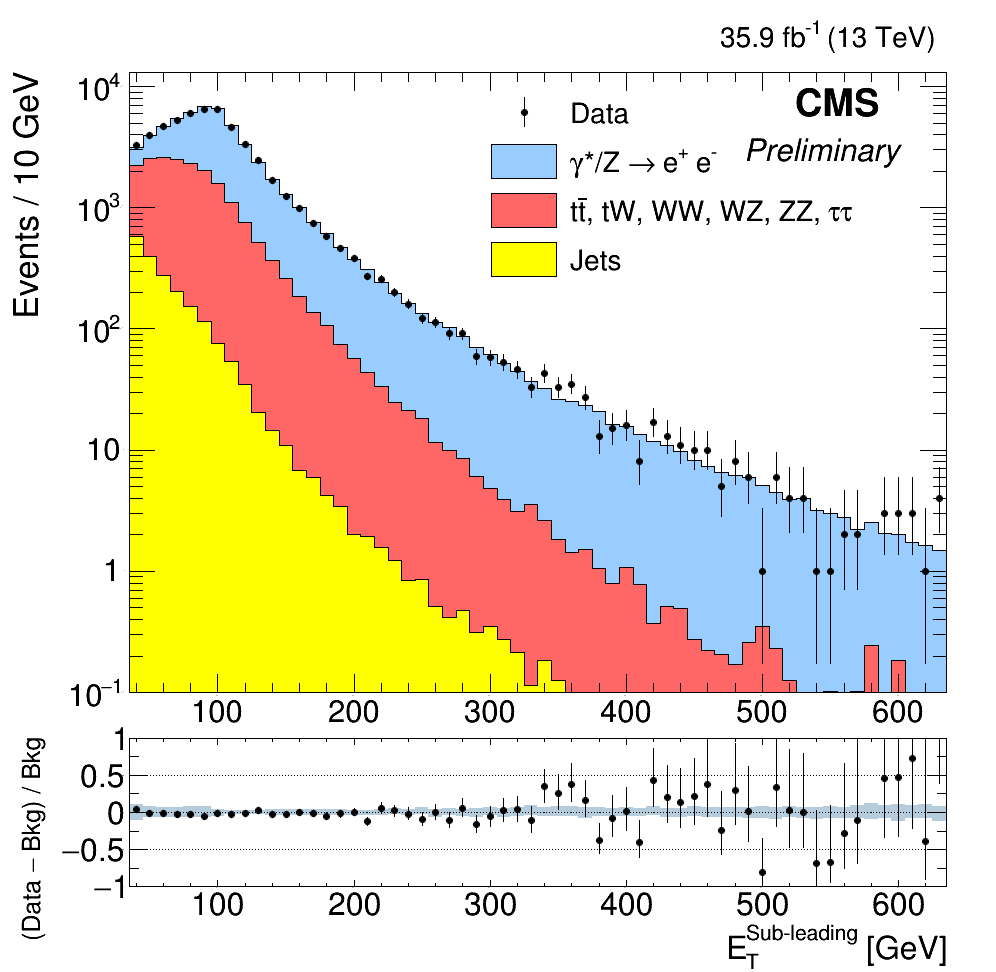
\includegraphics[width=0.32\textwidth]{figures/Zprime/2016/complementary/h_sub_Et.png}&
      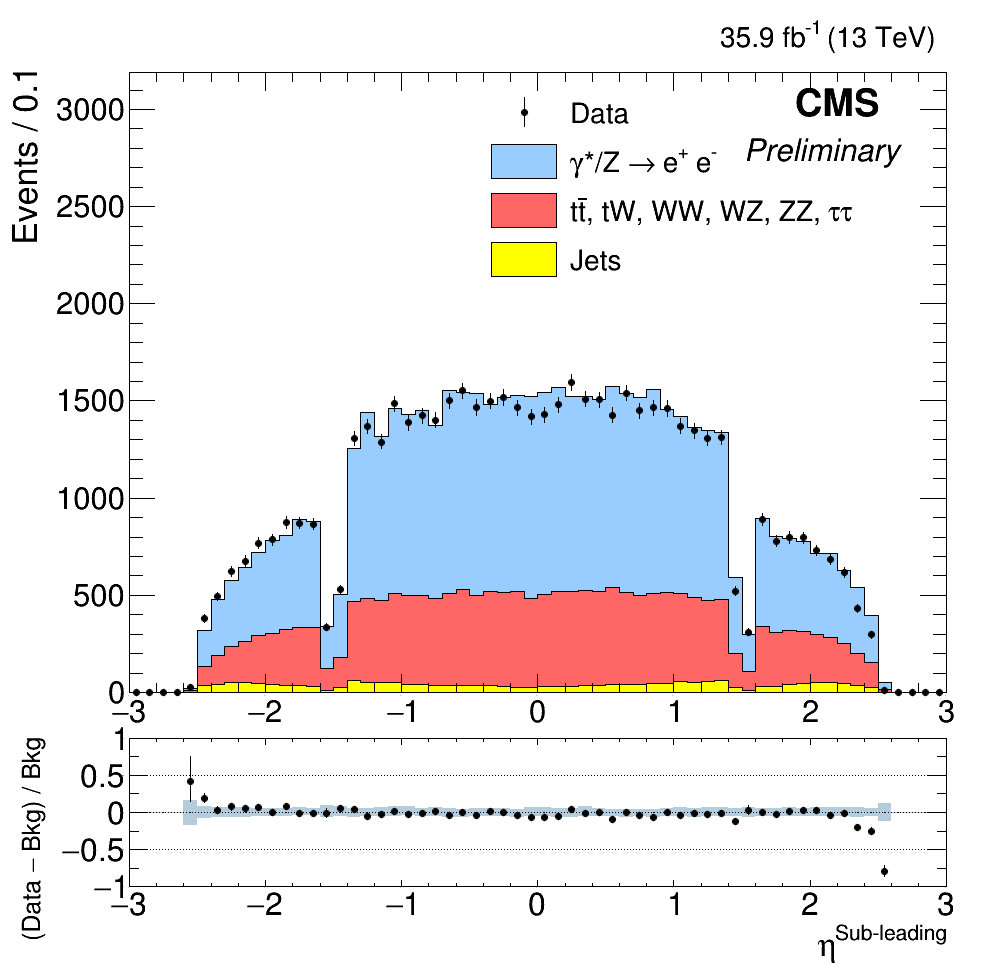
\includegraphics[width=0.32\textwidth]{figures/Zprime/2016/complementary/h_sub_eta.png}&
      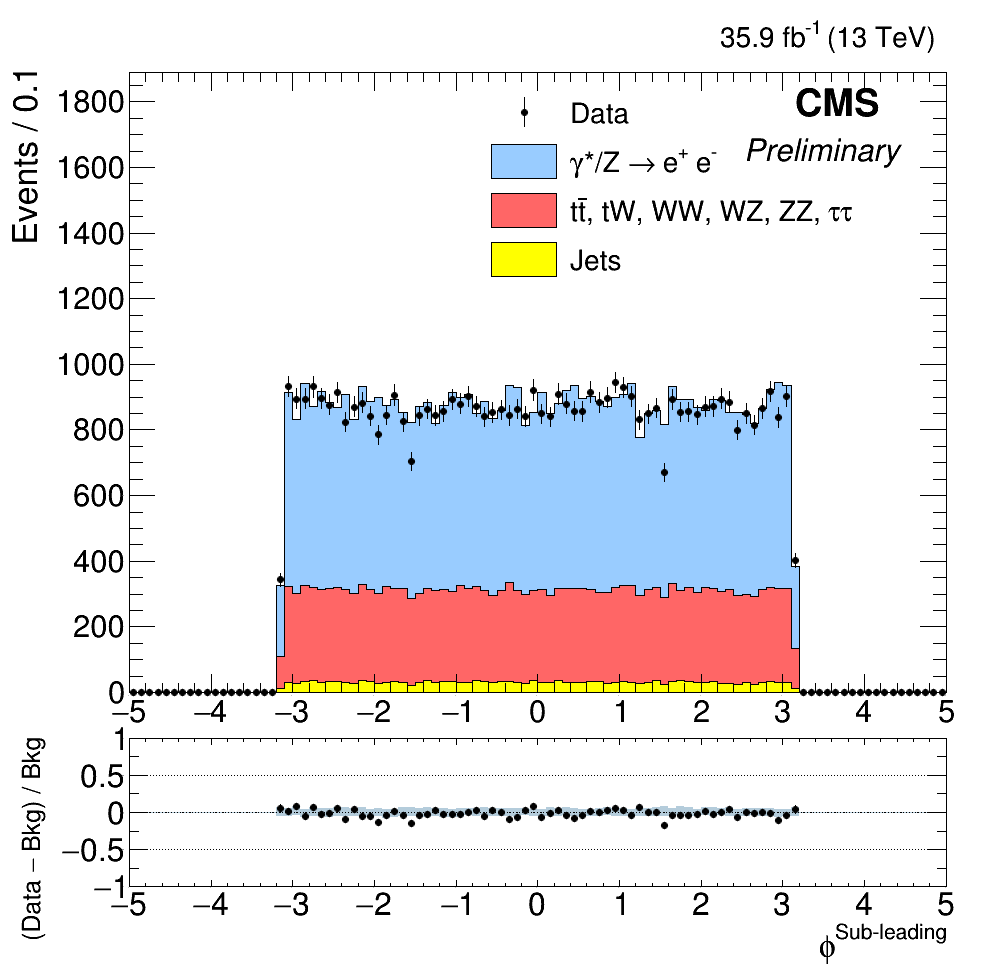
\includegraphics[width=0.32\textwidth]{figures/Zprime/2016/complementary/h_sub_phi.png}\\
      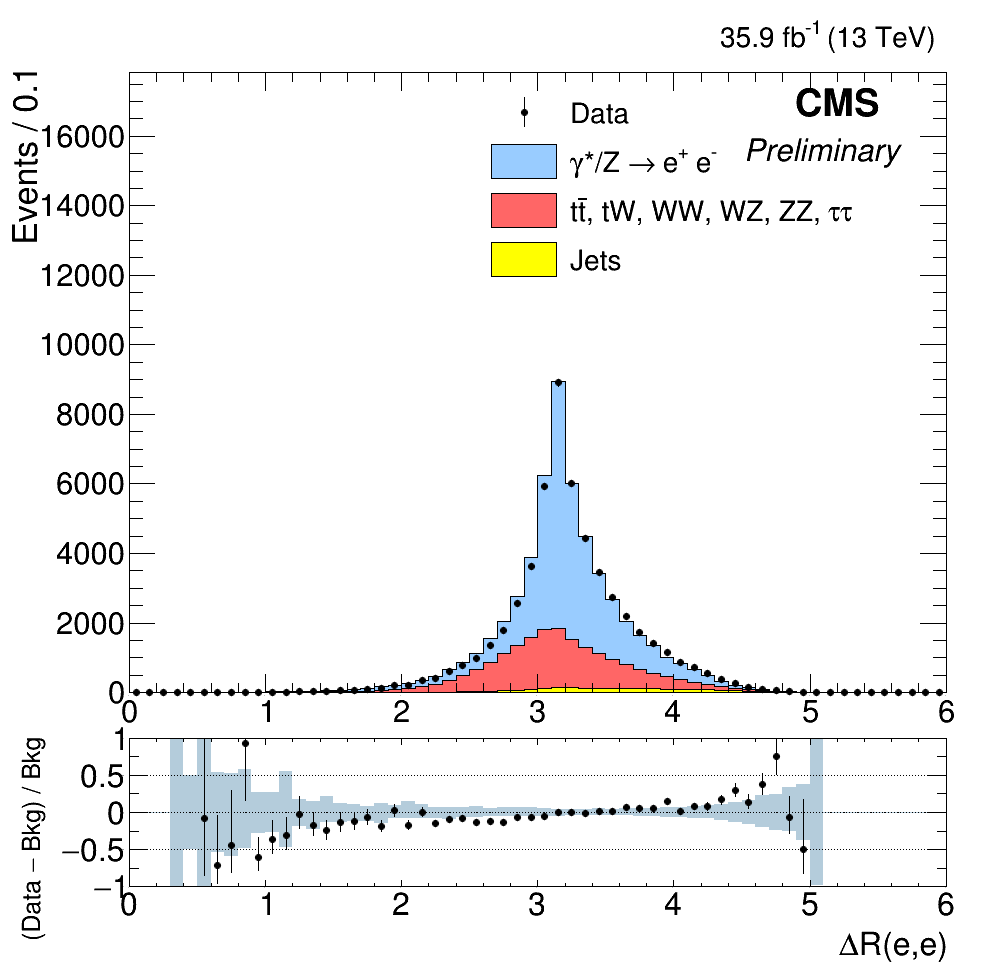
\includegraphics[width=0.32\textwidth]{figures/Zprime/2016/complementary/h_DR_ll.png}&
      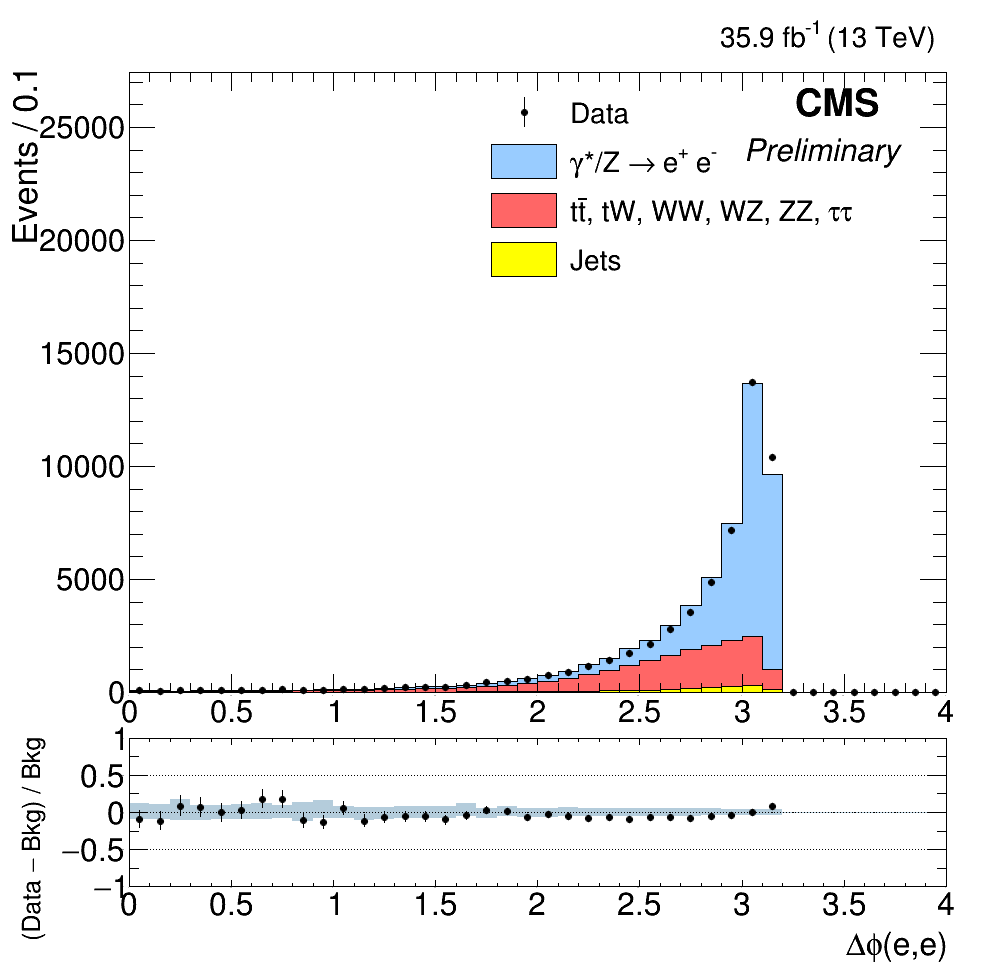
\includegraphics[width=0.32\textwidth]{figures/Zprime/2016/complementary/h_Dphi_ll.png}&
      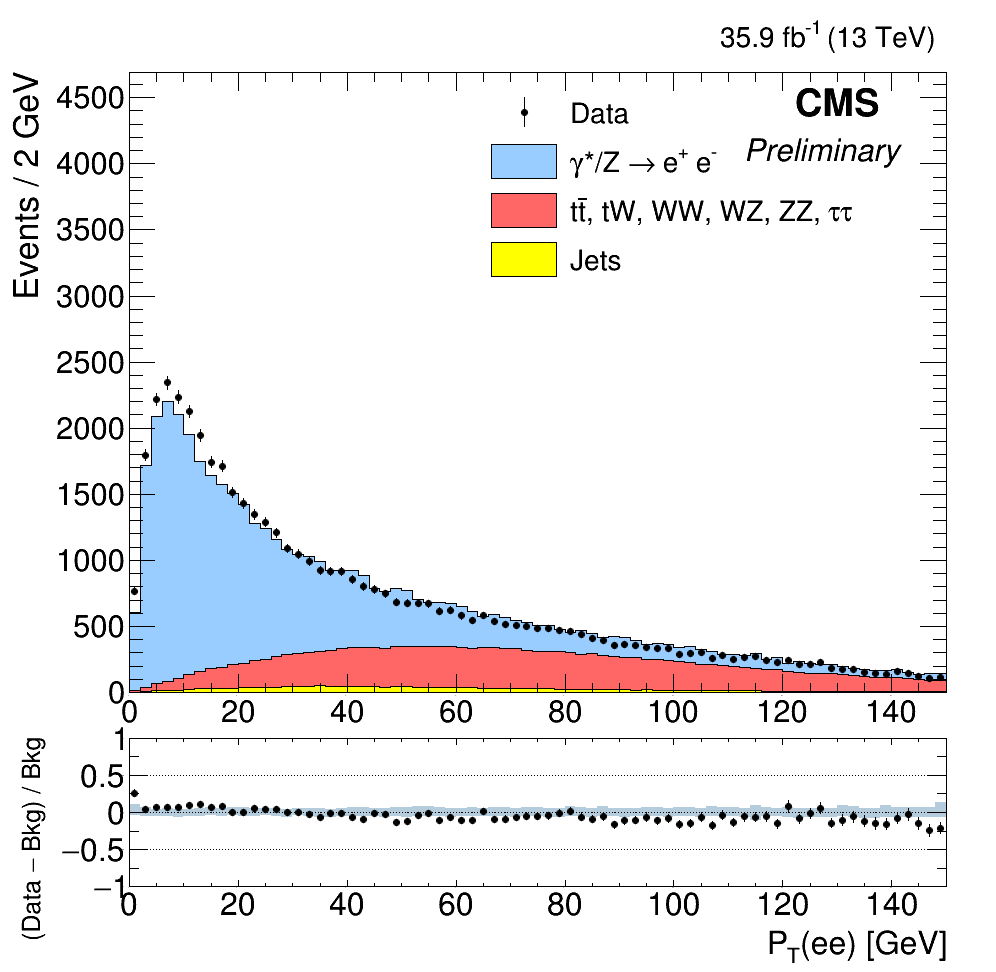
\includegraphics[width=0.32\textwidth]{figures/Zprime/2016/complementary/h_Ptll.png}\\
    \end{tabular}
    \caption{The distributions of invariant mass of two electrons in barrel-barrel, barrel-endcap and barrel-barrel + barrel-endcap (first row), $E_{T}$, $\eta$ and $\phi$ of leading electron (second row) and $E_{T}$, $\eta$ and $\phi$ of sub-leading electron (third row),$\Delta R$, $\Delta\phi$ between two electrons and $P_{T}$ of Z (fourth row) in 2016.
    \label{fig:complementary_2016}}
  \end{center}
\end{figure}

\begin{figure}[ht]
  \begin{center}
    \begin{tabular}{ccc}
      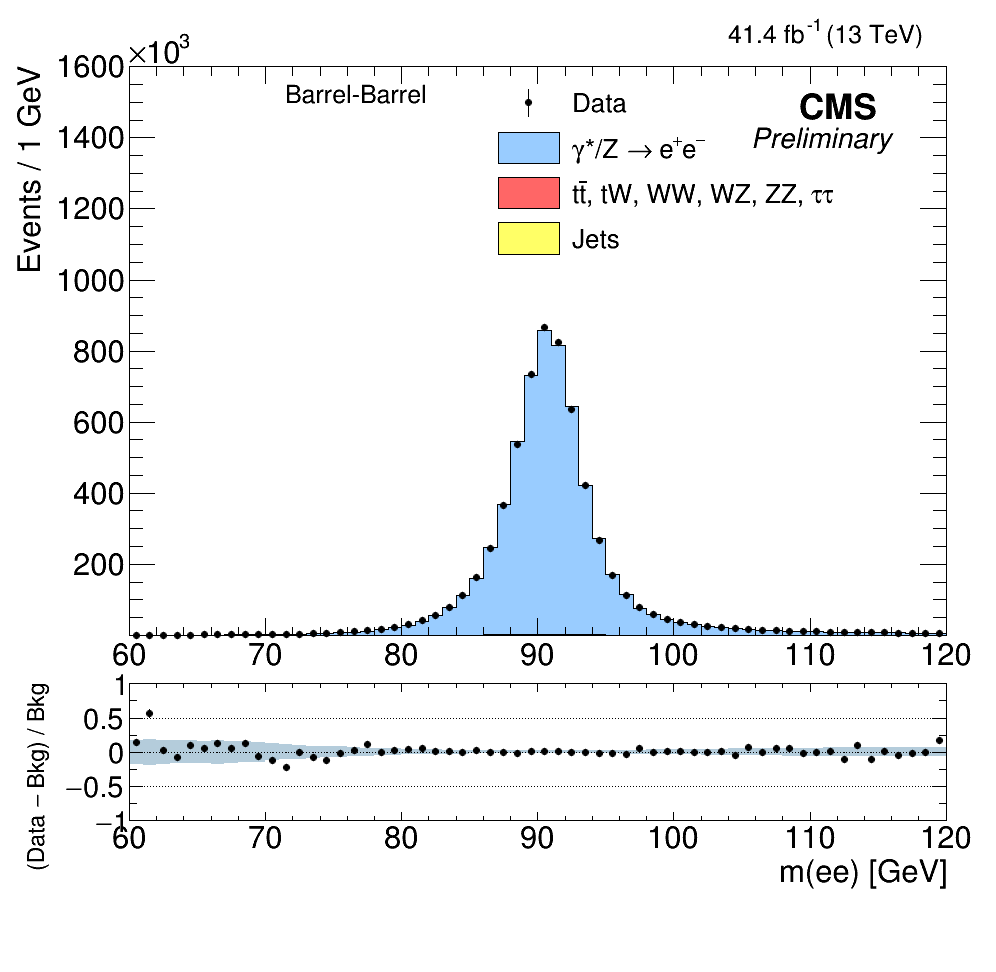
\includegraphics[width=0.32\textwidth]{figures/Zprime/2017/complementary/h_mee_Zpeak_BB.png}&
      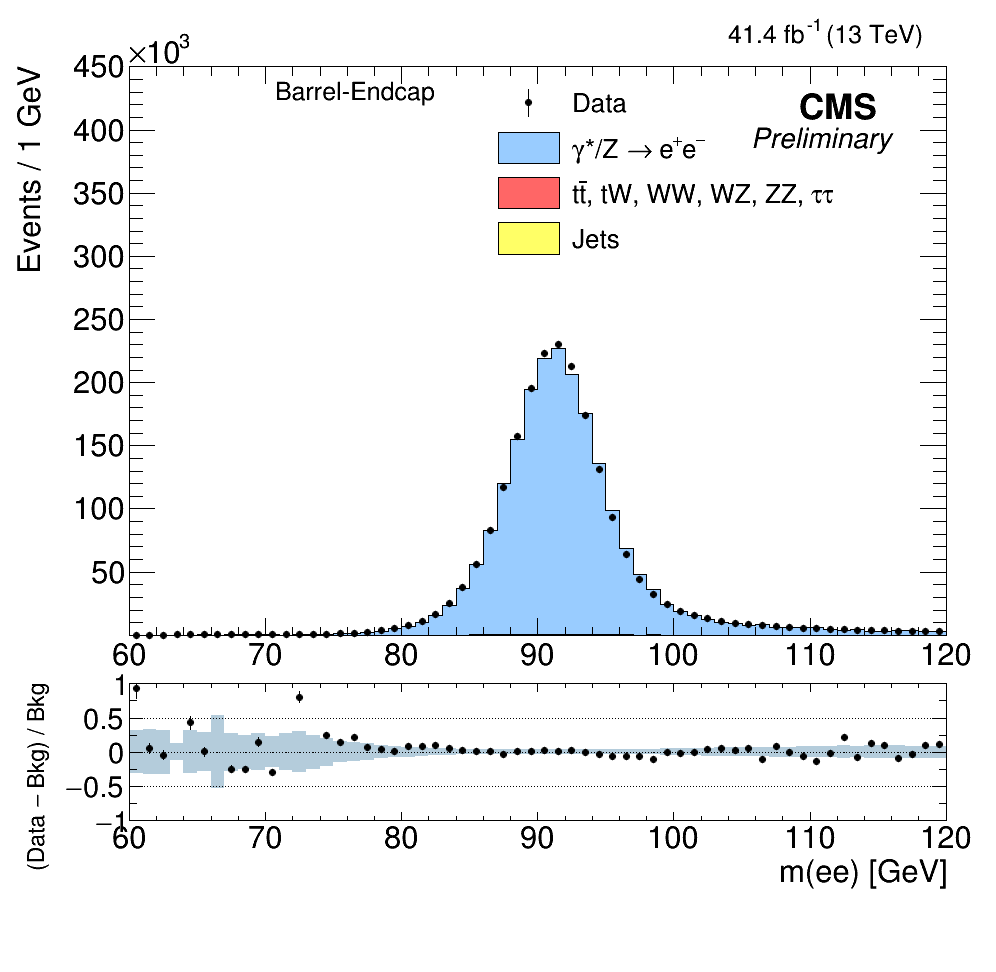
\includegraphics[width=0.32\textwidth]{figures/Zprime/2017/complementary/h_mee_Zpeak_BE.png}&
      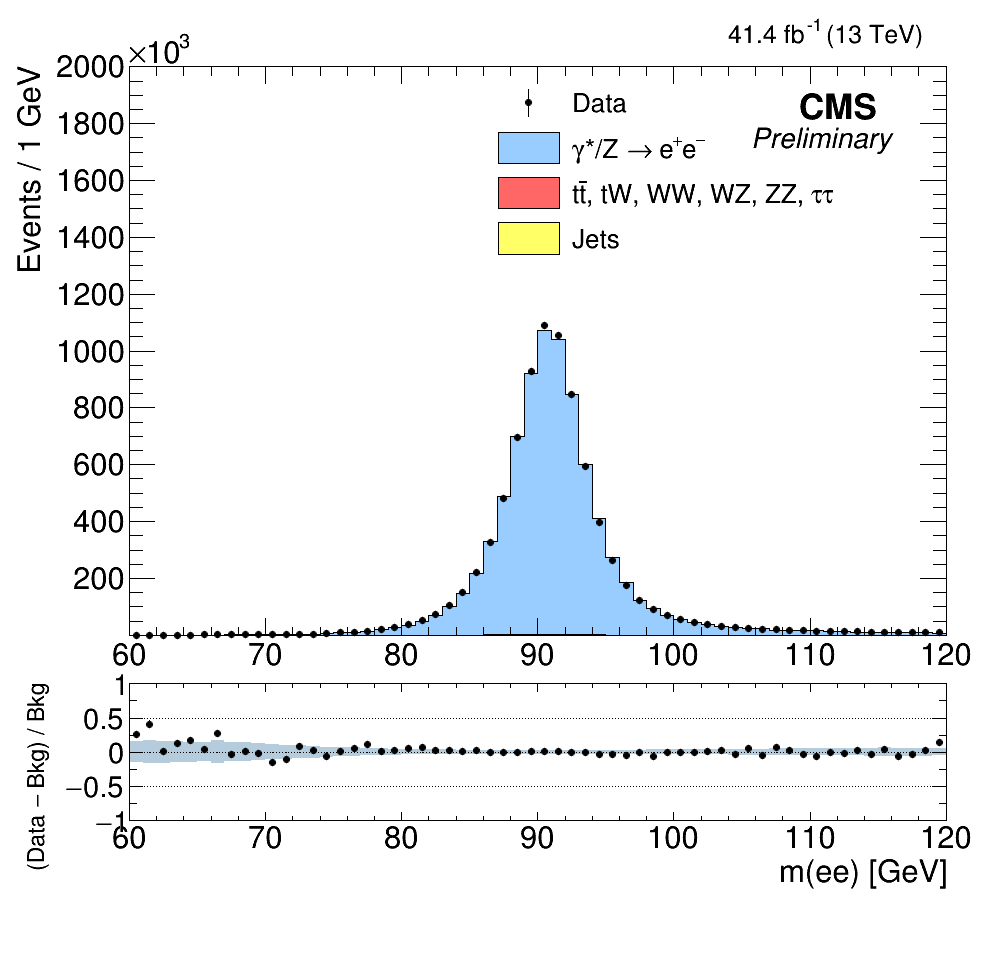
\includegraphics[width=0.32\textwidth]{figures/Zprime/2017/complementary/h_mee_Zpeak.png}\\
      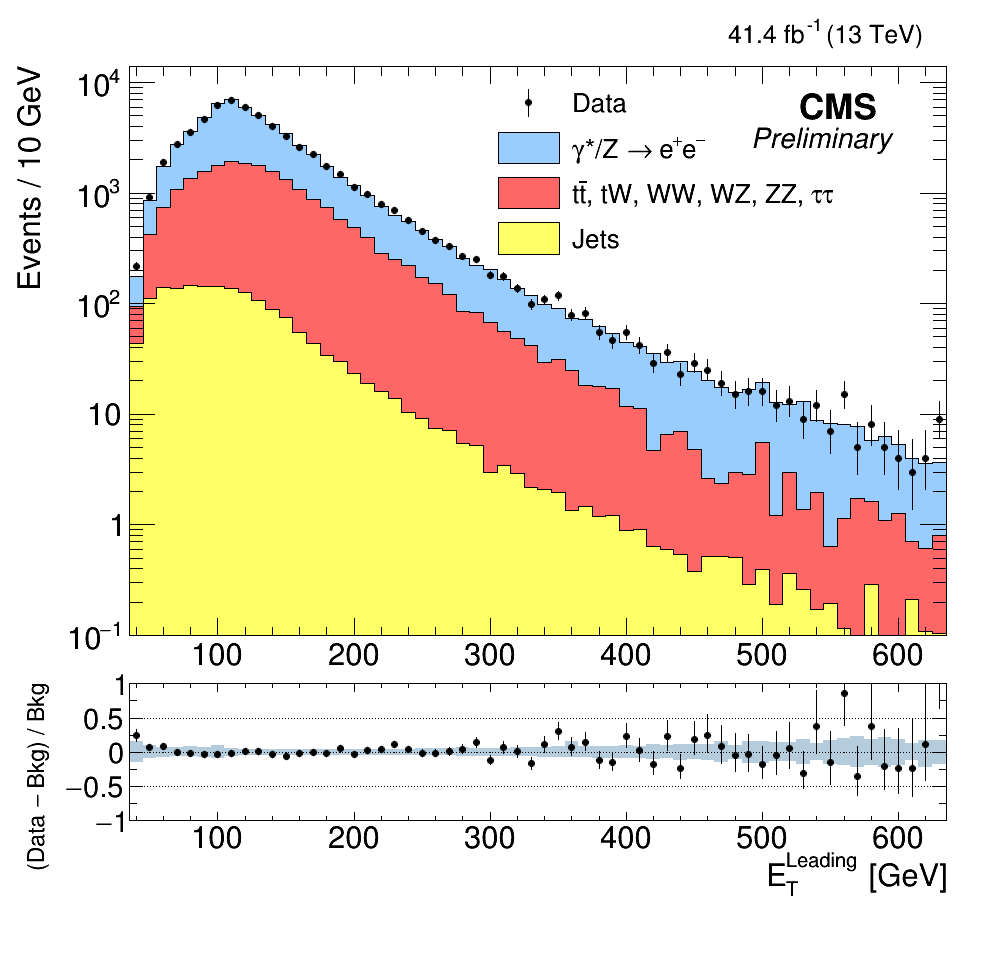
\includegraphics[width=0.32\textwidth]{figures/Zprime/2017/complementary/h_led_Et.png}&
      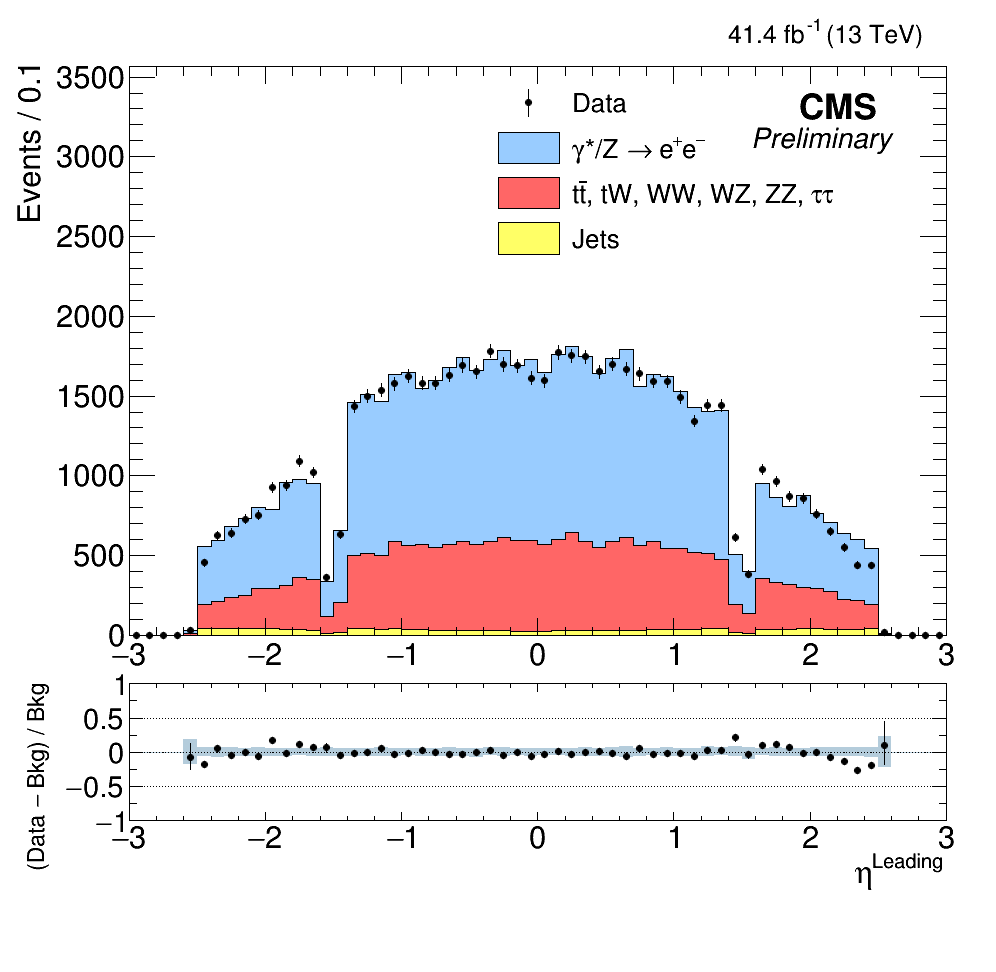
\includegraphics[width=0.32\textwidth]{figures/Zprime/2017/complementary/h_led_eta.png}&
      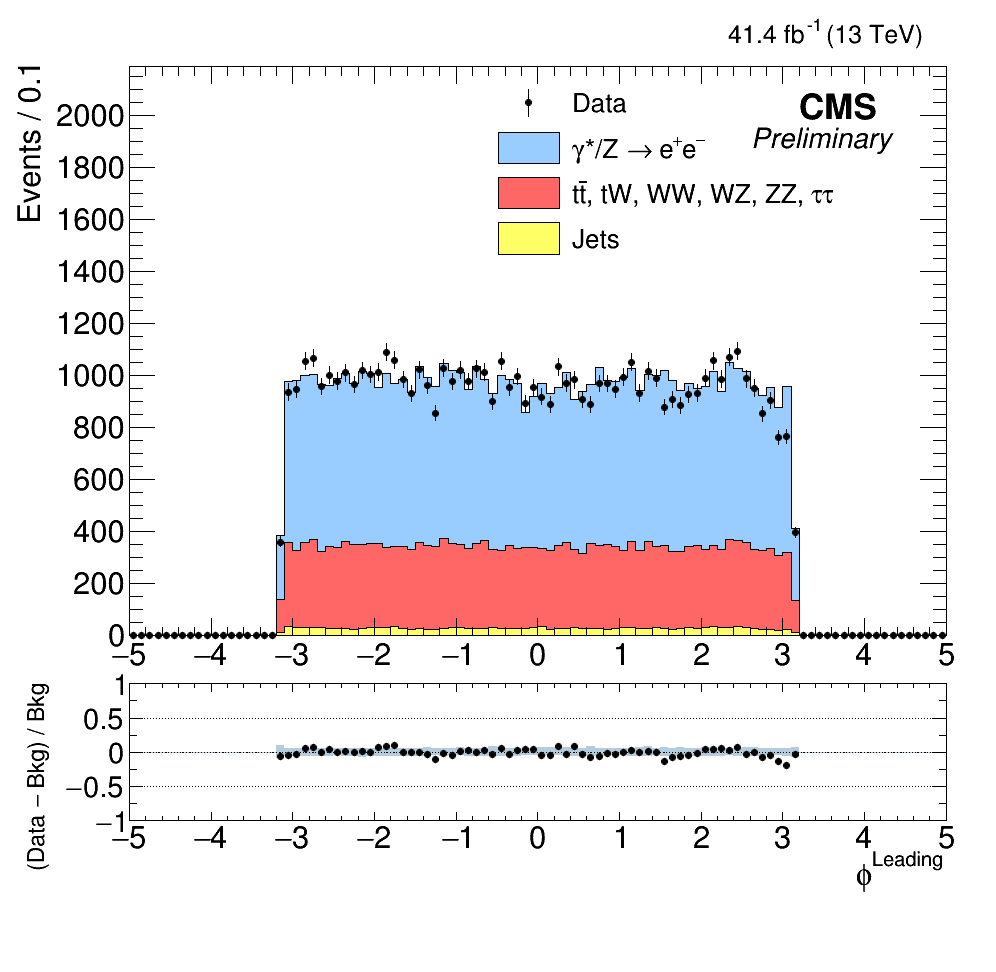
\includegraphics[width=0.32\textwidth]{figures/Zprime/2017/complementary/h_led_phi.png}\\
      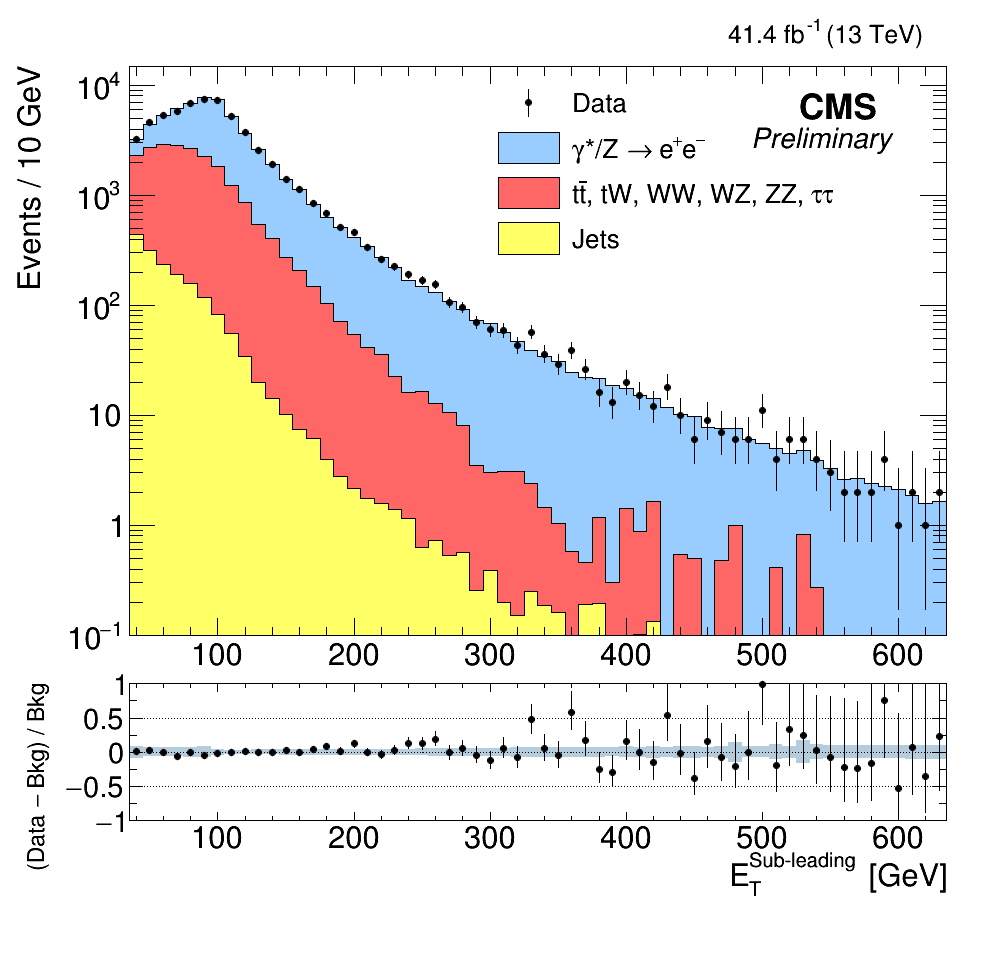
\includegraphics[width=0.32\textwidth]{figures/Zprime/2017/complementary/h_sub_Et.png}&
      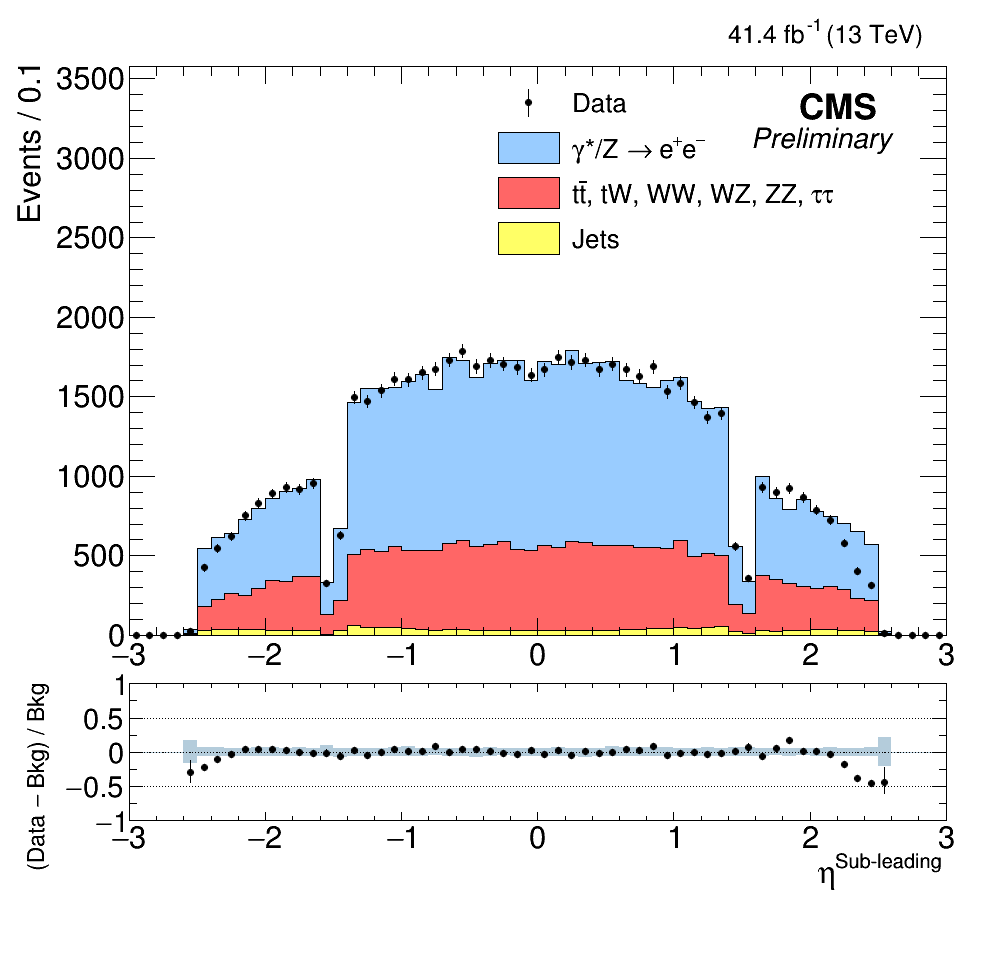
\includegraphics[width=0.32\textwidth]{figures/Zprime/2017/complementary/h_sub_eta.png}&
      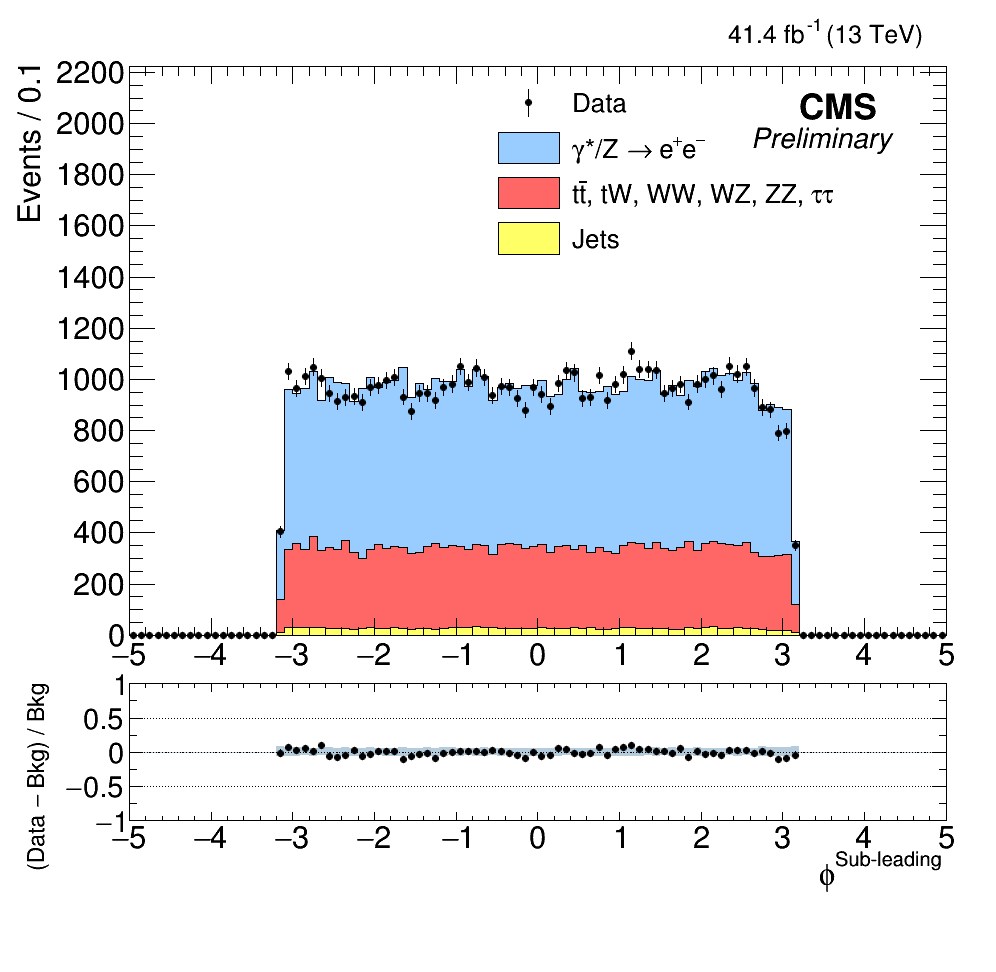
\includegraphics[width=0.32\textwidth]{figures/Zprime/2017/complementary/h_sub_phi.png}\\
      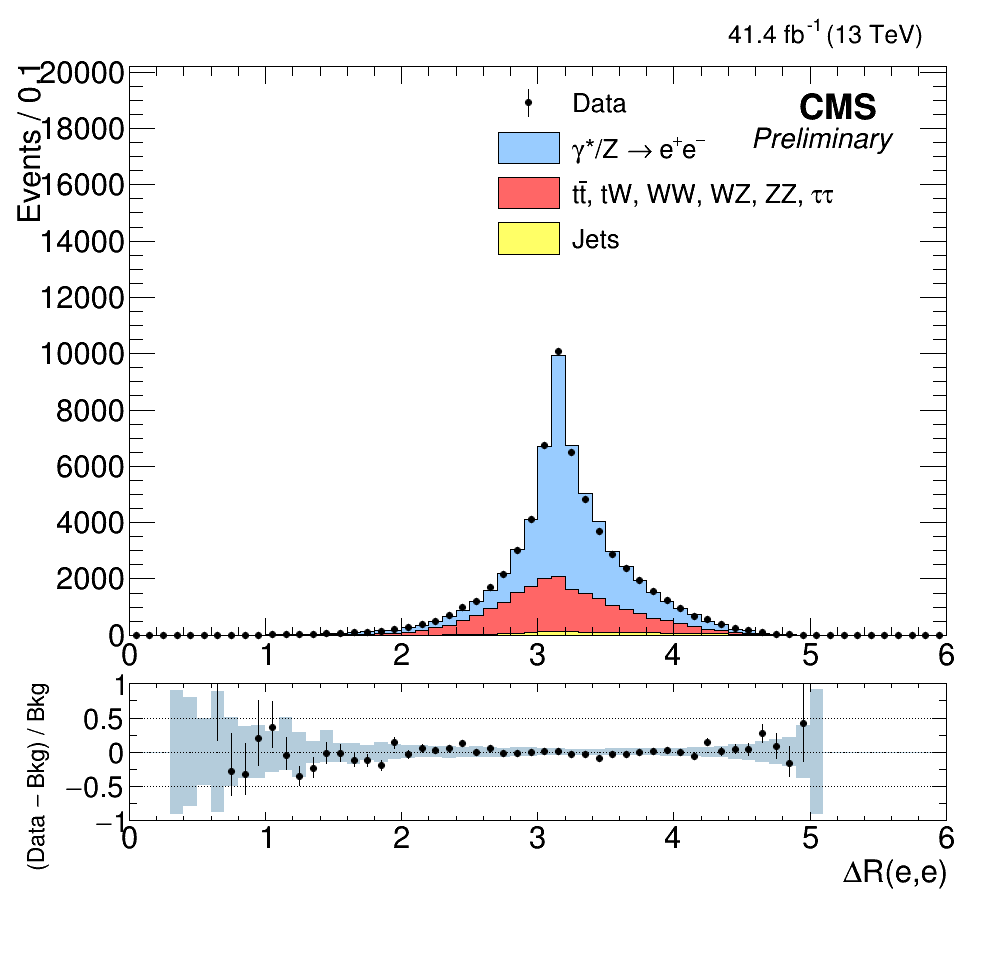
\includegraphics[width=0.32\textwidth]{figures/Zprime/2017/complementary/h_DR_ll.png}&
      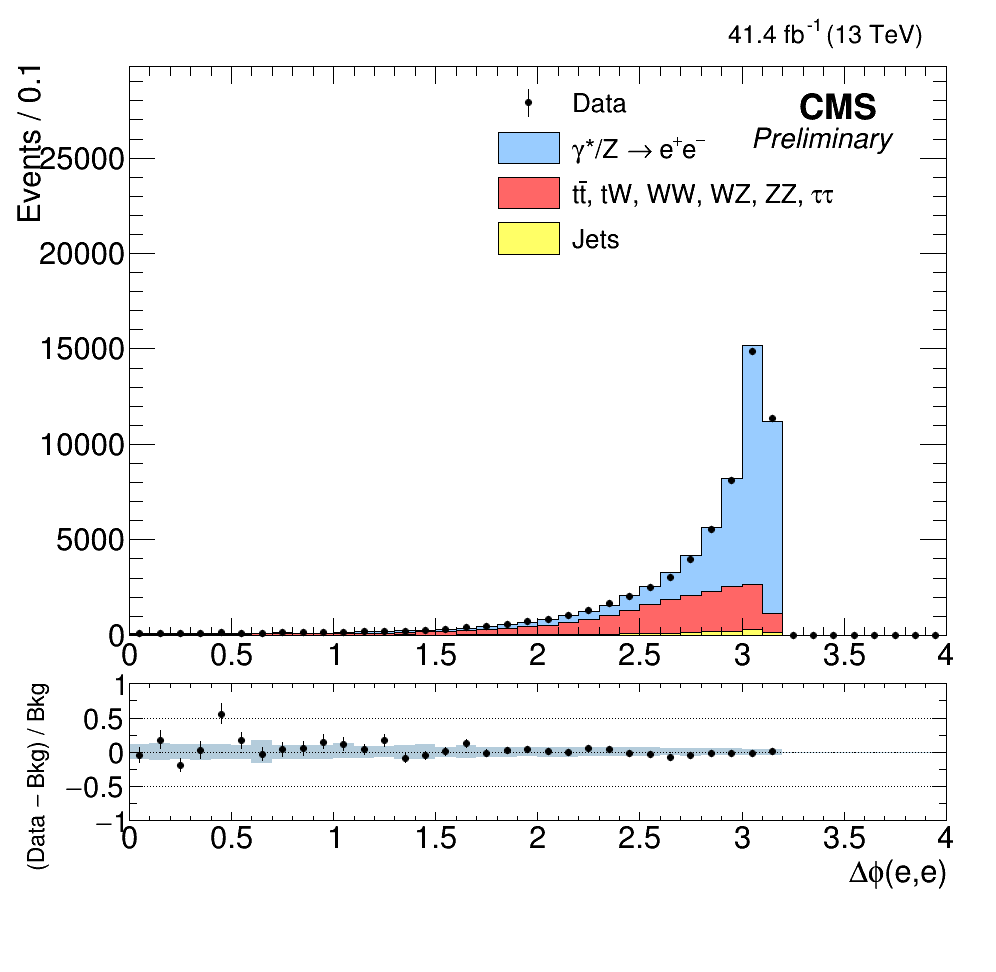
\includegraphics[width=0.32\textwidth]{figures/Zprime/2017/complementary/h_Dphi_ll.png}&
      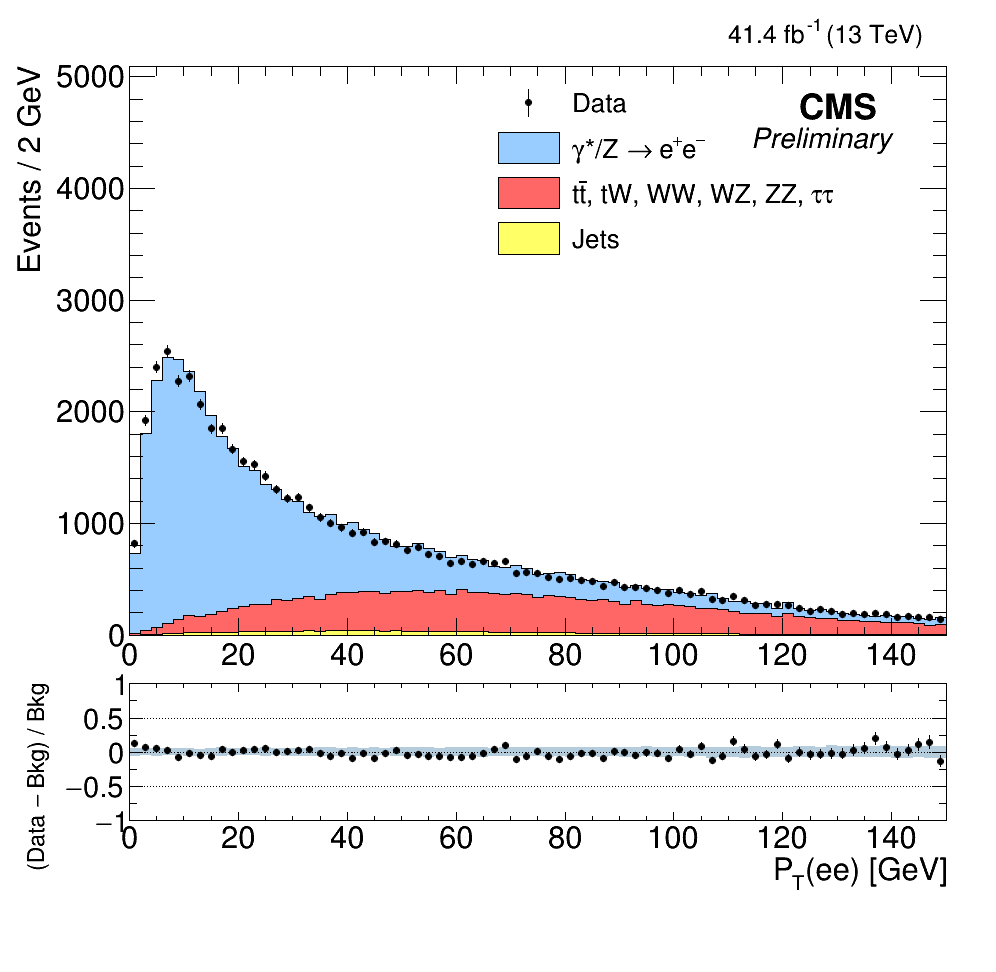
\includegraphics[width=0.32\textwidth]{figures/Zprime/2017/complementary/h_Ptll.png}\\
    \end{tabular}
    \caption{The distributions of invariant mass of two electrons in barrel-barrel, barrel-endcap and barrel-barrel + barrel-endcap (first row), $E_{T}$, $\eta$ and $\phi$ of leading electron (second row) and $E_{T}$, $\eta$ and $\phi$ of sub-leading electron (third row),$\Delta R$, $\Delta\phi$ between two electrons and $P_{T}$ of Z (fourth row) in 2017.
    \label{fig:complementary_2017}}
  \end{center}
\end{figure}


\clearpage

